Photon candidates are required to have $E_{T} > 20 \GeV$ and be in the fiducial Barrel region or Endcap regions,
defined by $|\eta|<1.4442$ and $1.566<|\eta|<2.5$, respectively.
The photon candidates are also required to be separated from the closest lepton (electron or muon) by at least $\DR(\PGg, \Pl) > 0.5$,
which highly suppresses the contribution from FSR,
and is orthogonal to the selection used for lepton FSR recovery (see Section \ref{sec:FSRphotons}).

Different strategies are used to identify prompt (produced at the primary vertex) and isolated
electrons and photons, and separate them from background sources.
The most important background to prompt photons arises from jets fragmenting mainly into light neutral mesons
such as \Pgpz or \PGh, which promptly decay to two photons.
For the energy range of interest, the meson is significantly boosted, such that the two photons from the decay are nearly collinear
and are difficult to distinguish from a single-photon incident on the calorimeter.
%% Different working points are defined to identify either electrons or photons,
%% corresponding to identification efficiencies of approximately 70, 80, and 90 \%, respectively.
%% In all cases data and simulation efficiencies are compatible within 1-5 \% over the full $\eta$ and \ET ranges for electrons and photons.

Both a cut-based and a MVA-based ID are employed and compared in the analysis.
Each has its own advantages and disadvantages.
Due to its nature, the cut-based ID can be easily inverted by reversing only one or a few of its cuts.
On the other hand, MVA-based ID is more effective at discriminating between signal and background, providing a higher signal-to-noise ratio.

\paragraph{Identification variables\\}
One of the most efficient ways to reject photon backgrounds is the use of isolation energy sums,
a generic class of discriminating variables that are constructed from the sum of the reconstructed energy in a cone around photons in different subdetectors.
%% For this purpose, it is convenient to define cones in terms of an $\eta-\phi$ metric;
%% the distance with respect to the reconstructed photon direction is defined by \DR.
A veto region inside the cone is defined, to ensure that the energy from the photon itself is not included in this sum.

Photon isolation exploits the information provided by the PF event reconstruction (Section \ref{sec:ParticleFlow}).
The isolation variables are obtained by summing the transverse momenta of charged hadrons ($I_{ch}$), photons ($I_\PGg$), and neutral hadrons ($I_n$),
inside an isolation cone of $\DR = 0.3$ with respect to the electron or photon direction.
The larger the energy of the incoming electrons or photons, the larger the amount of energy spread around its direction in the various subdetectors.
For this reason, the thresholds applied on the isolation quantities are frequently parameterised as a function of the particle \ET.

The isolation variables are corrected to mitigate the contribution from pileup.
This contribution in the isolation region is estimated as $\rho A_{eff}$,
where $\rho$ is the median of the transverse energy density per unit area in the event
and $A_{eff}$ is the area of the isolation region weighted by a factor that accounts for the dependence of the pileup transverse energy density on the object $\eta$ \cite{CMS:electron-performance-2015}.
The quantity $\rho A_{eff}$ is subtracted from the isolation quantities.

The distributions of $I_\PGg$ before % after?
the $\rho$ corrections are shown in Figure~\ref{fig:Iph_CR2P2F} for photons in the EB and EE.

\begin{figure}
\subfigure [Barrel] {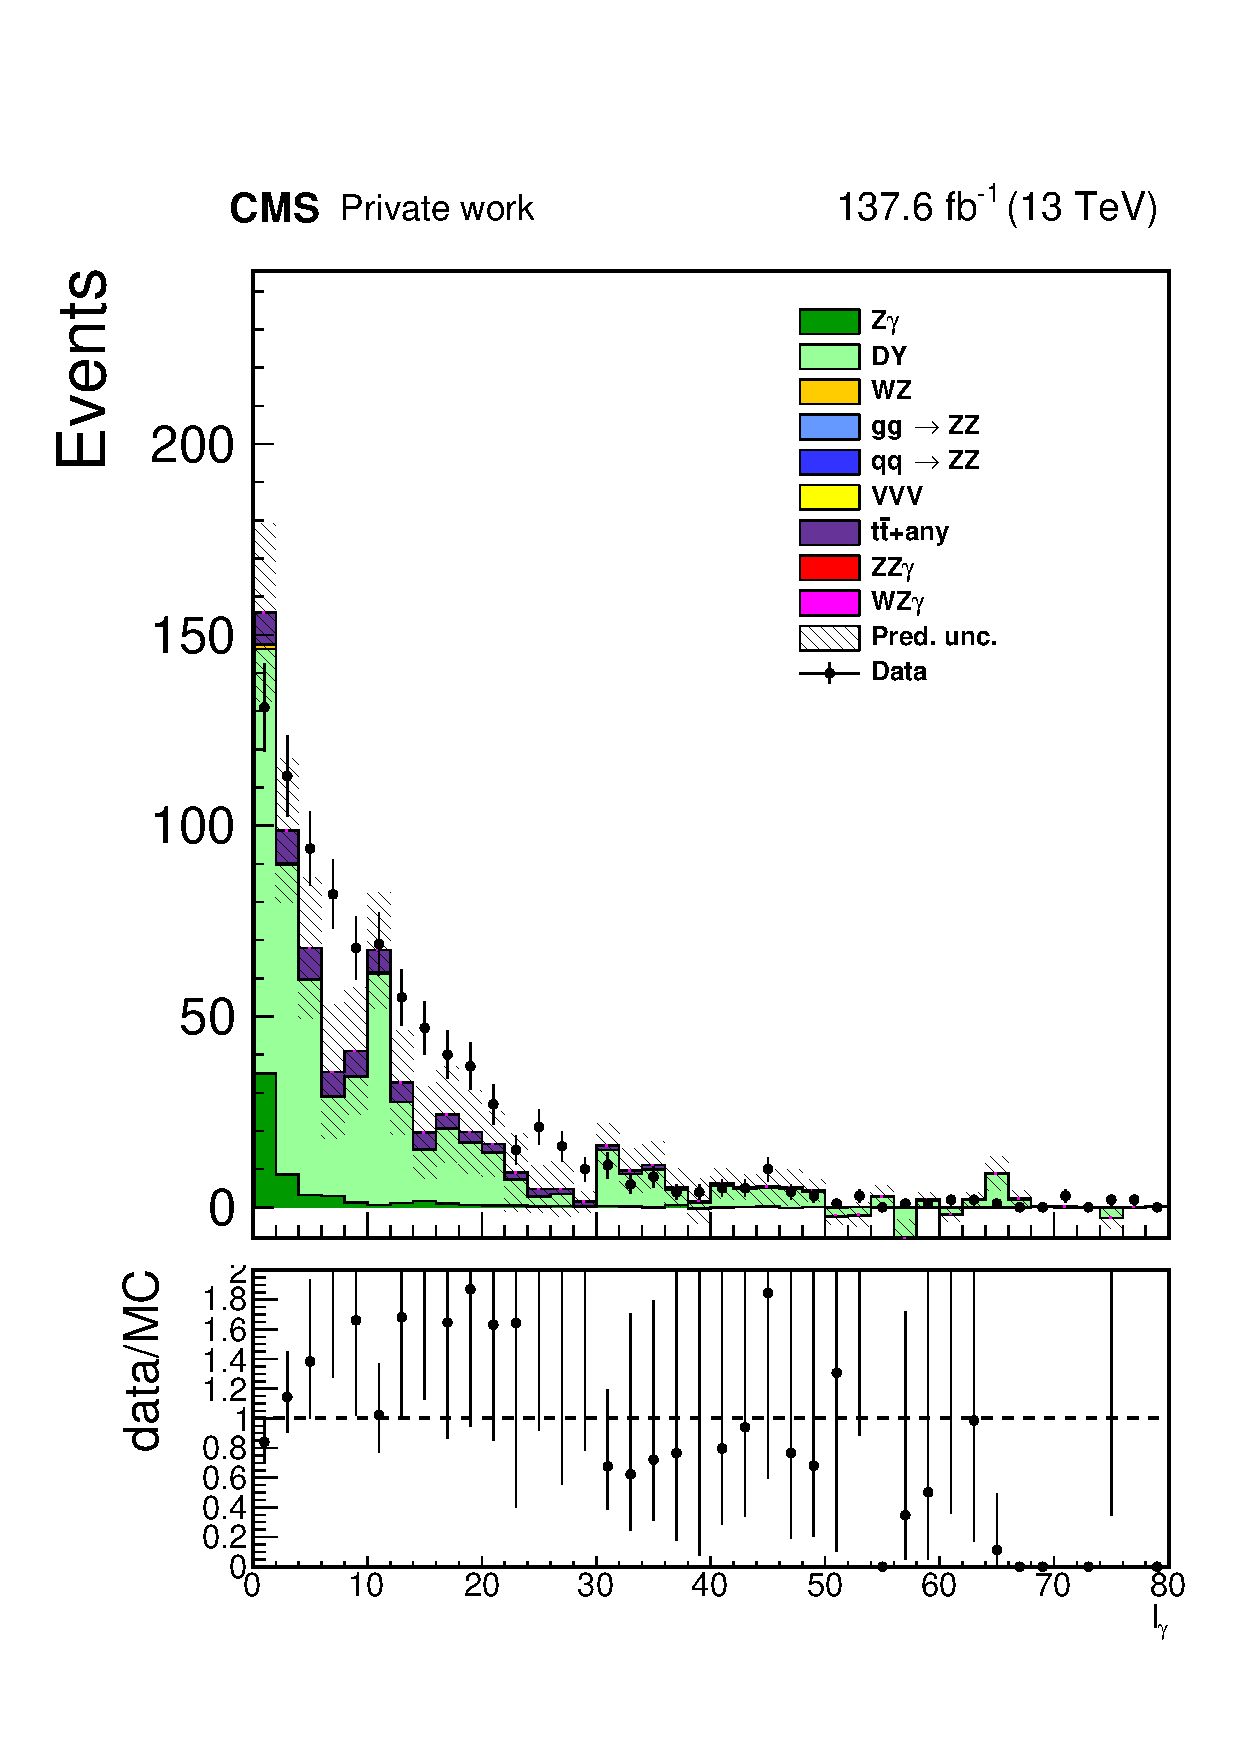
\includegraphics[width=.5\textwidth]{Figures/VVGammaAnalyzer_noLFR/Run2/fullMC/CR2P2F/kinPh_phIso_EB_pow.pdf}}%
\subfigure [Endcap] {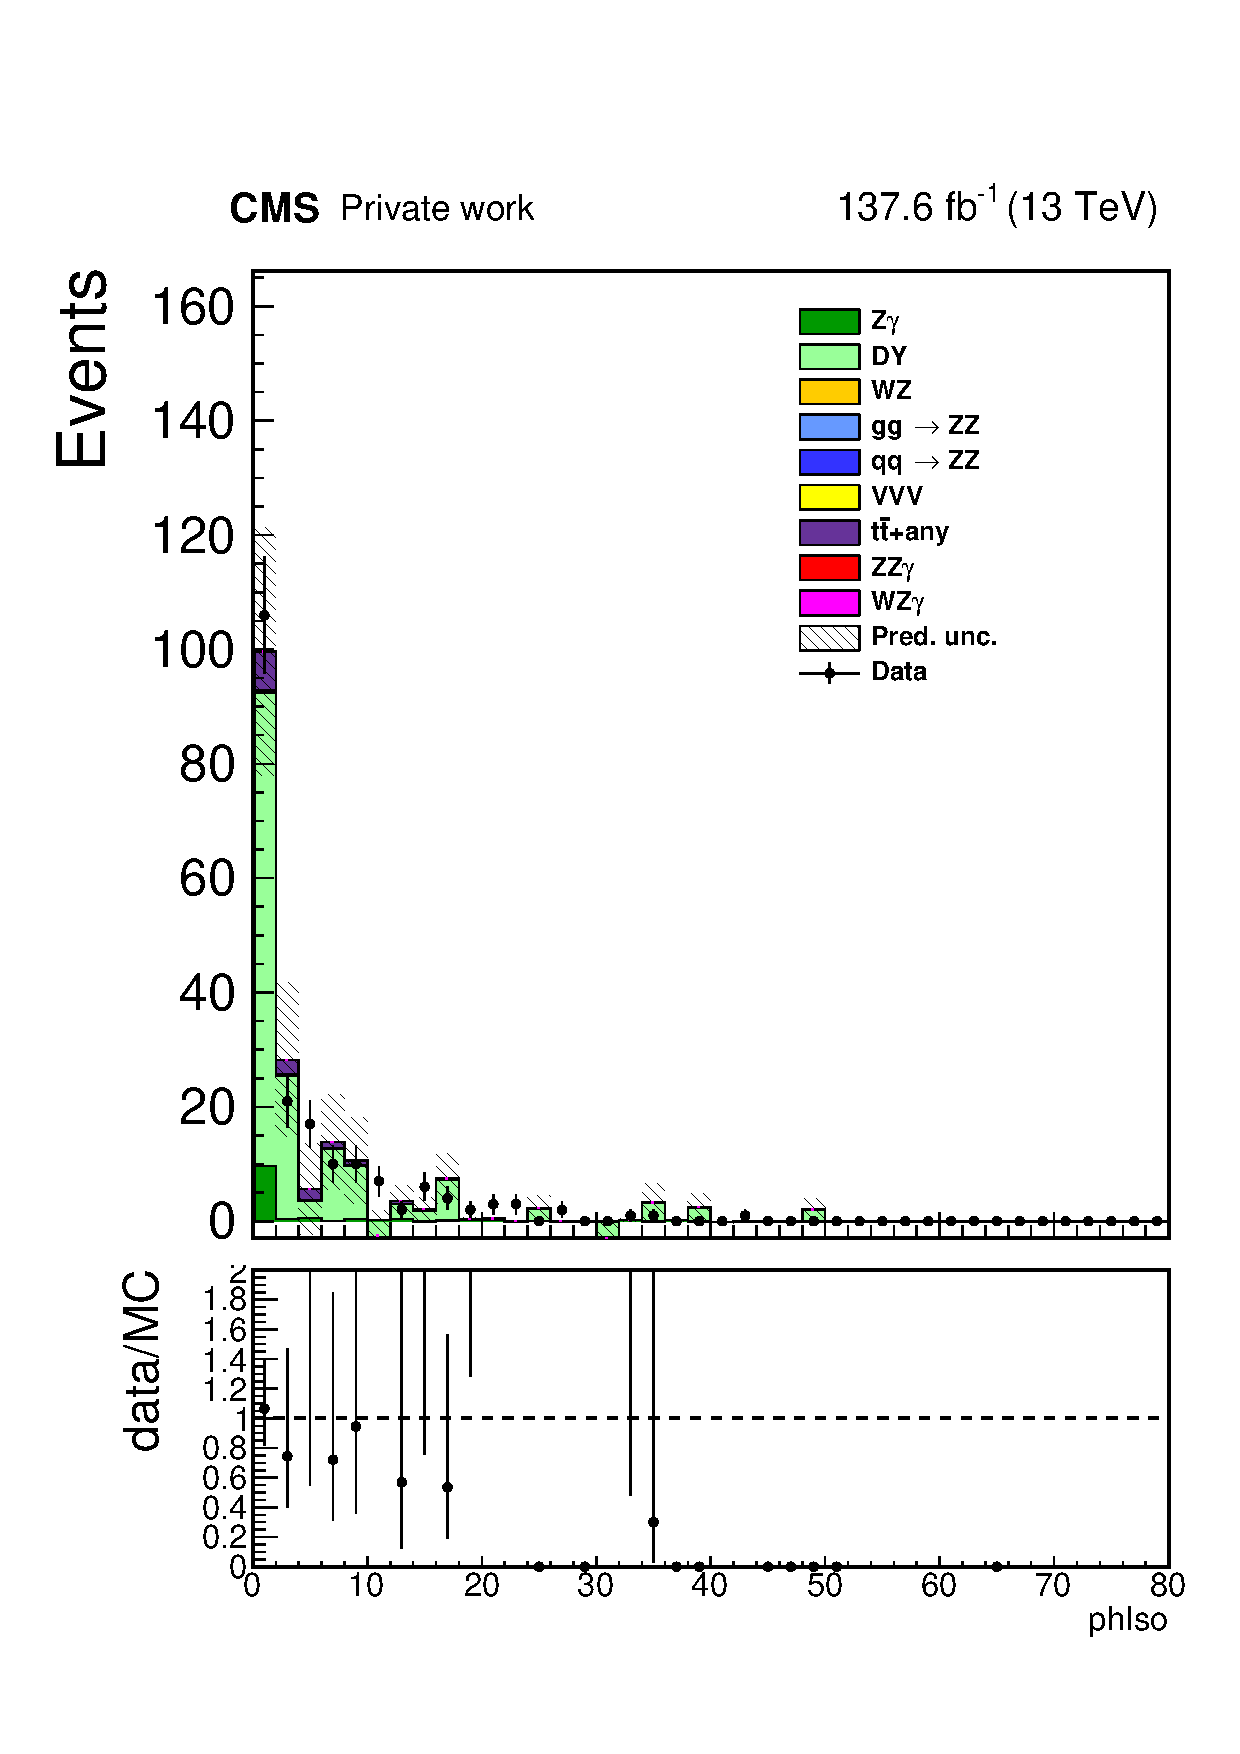
\includegraphics[width=.5\textwidth]{Figures/VVGammaAnalyzer_noLFR/Run2/fullMC/CR2P2F/kinPh_phIso_EE_pow.pdf}}
\caption{The PF photon isolation ($I_\PGg$), before the $\rho$ correction, in a cone defined by $\DR = 0.3$ for photons in the EB (left) and in the EE (right).
The events belong to the leptonic control region CR2P2F (see Section \ref{sec:fake_leptons}).
The lower panels display the ratio of the data to the simulation.}
\label{fig:Iph_CR2P2F}
\end{figure}

Another method to reject jets with high electromagnetic content exploits the shape of the electromagnetic shower in the ECAL.
Even if the two photons from neutral hadron decays inside a jet cannot be fully resolved, a wider shower profile is expected, on average,
compared with a single incident electron or photon.
This is particularly true along the $\eta$ axis of the cluster, since the presence of the material combined with the effect of the magnetic field
reduce the discriminating power resulting from the $\phi$ profile of the shower. 
In particular, the following two variables have high discriminating power.

The hadronic over electromagnetic energy ratio ($H/E$) is defined as the ratio between the energy deposited in the HCAL in a cone of radius $\DR = 0.15$
around the supercluster direction and the energy of the photon candidate.
\sieie, the second moment of the log-weighted distribution of crystal energies in $\eta$,
calculated in the $5 \times 5$ matrix around the most energetic crystal in the SC and rescaled to units of crystal size.
The mathematical expression is given below:
\begin{equation}
\label{eq:sieie}
\sieie \mathdefined \sqrt{ \frac{\sum_i^{5 \times 5} w_i(\eta_i - \bar{\eta}_{5 \times 5})}{\sum_i^{5 \times 5} w_i} }
\end{equation}
where $\eta_i$ is the pseudorapidity of the i-th crystal,
$\bar{\eta}_{5 \times 5}$ is the mean pseudorapidity of the $5 \times 5$ cells
and $w_i$ is a weight defined as $w_i = \mathrm{max}(0,\, 4.7 + \mathrm{ln}(E_i/E_{5 \times 5}))$,
which is nonzero if $E_i > 0.9\, \%\; E_{5 \times 5}$.
Looking at the numerator in Equation \ref{eq:sieie}, it is clear that \sieie is proportional to the distance between adjacent crystals,
which is 0.0175 in EB and varies from 0.0175 to 0.0 in EE.
Therefore, the spread of \sieie in EE is twice the one in EB.
The \sieie distribution is expected to be narrow for isolated electrons or photons, and broad for two-photon showers from meson decays.
The distributions of \sieie are shown in Figure \ref{fig:sieie_CR2P2F} for photons in the EB and EE.

\begin{figure}
\subfigure [Barrel] {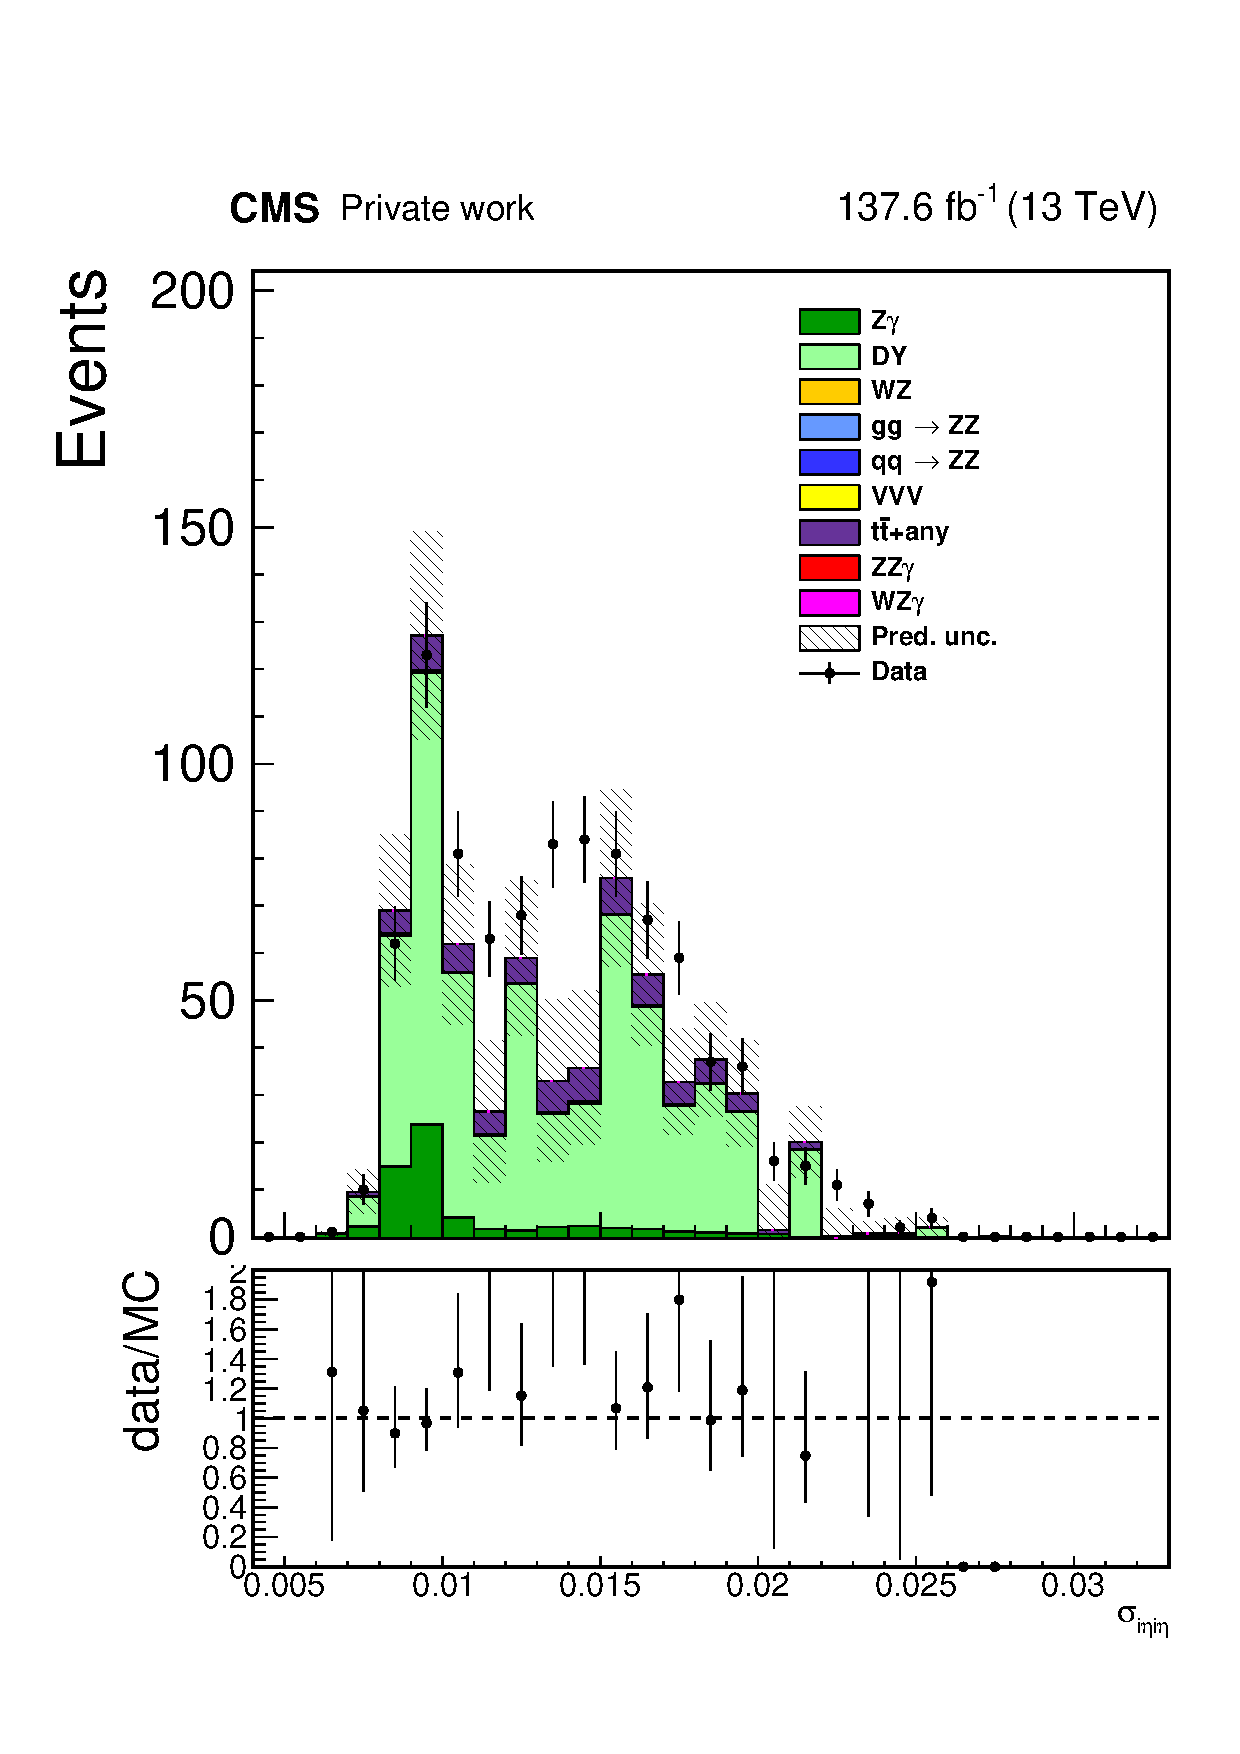
\includegraphics[width=.5\textwidth]{Figures/VVGammaAnalyzer_noLFR/Run2/fullMC/CR2P2F/kinPh_sieie_EB_pow.pdf}}%
\subfigure [Endcap] {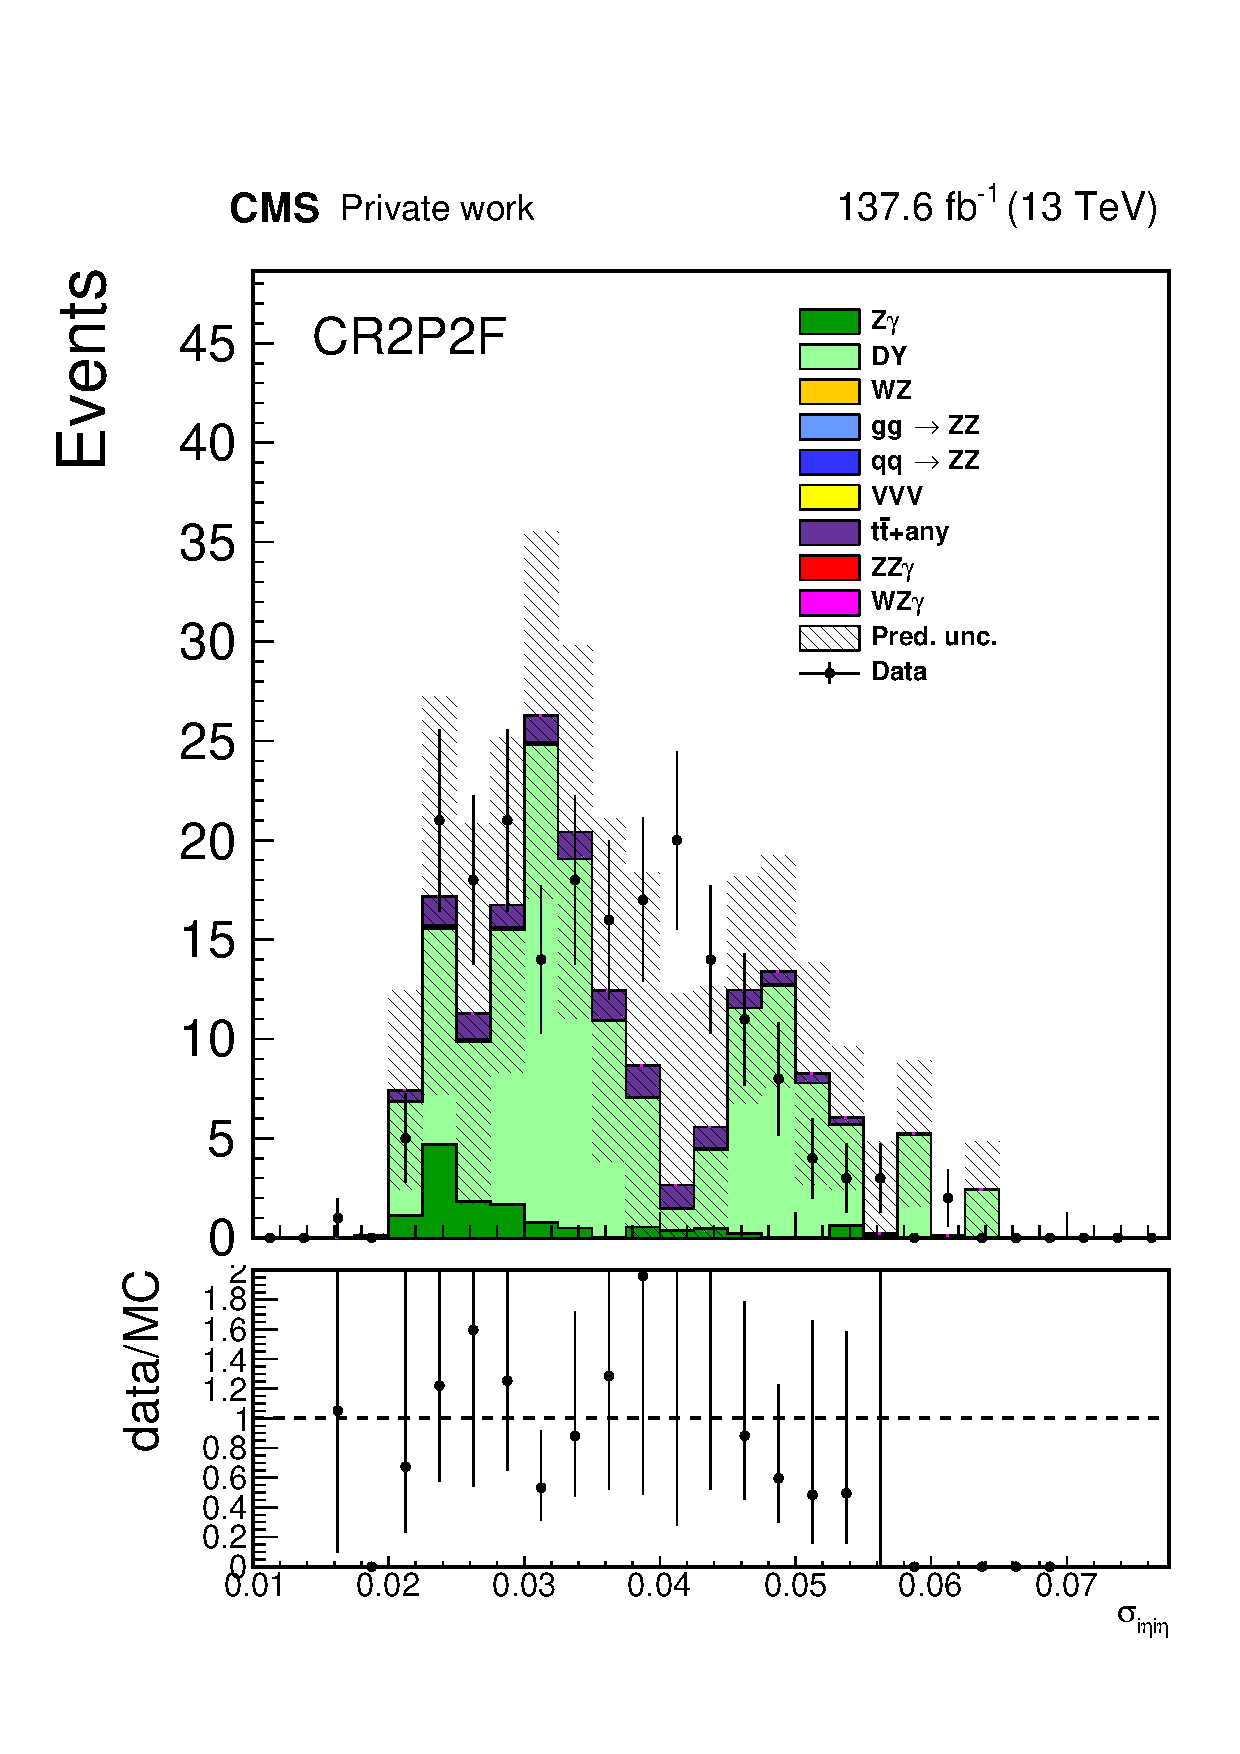
\includegraphics[width=.5\textwidth]{Figures/VVGammaAnalyzer_noLFR/Run2/fullMC/CR2P2F/kinPh_sieie_EE_pow.pdf}}
\caption{Distribution of \sieie for photons in the EB (left) and in the EE (right).
The events belong to the leptonic control region CR2P2F (see Section \ref{sec:fake_leptons}).
The lower panels display the ratio of the data to the simulation.}
\label{fig:sieie_CR2P2F}
\end{figure}

Another important variable is $R_9$, which is defined as the ratio between the energy contained in the $3 \times 3$ array of crystals,
centered around the most energetic crystal of the SC,
to the total energy of the supercluster.

\paragraph{Cut-based ID\\}
The cut-based photon ID~\cite{CMS:EGM-17-001} uses 5 variables: $H/E$, \sieie, $I_{ch}^{corr}$, $I_{n} ^{corr}$ and $I_{\PGg} ^{corr}$.
The Loose working point, shown in Table~\ref{tab:VPhotonID}, is selected for this analysis.
It provides 90\,\% efficiency on signal photons with 86\,\% (77\,\%) background rejection in the Barrel (Endcap).
The efficiency in data is well modelled in simulation, and the ratio between the two, shown in Figure \ref{fig:phEffSF}, is within 5\,\% from unity.
This ratio is referred as Scale Factor (SF), and is applied to simulation to correct for the residual mismodelling and avoid biasing the results.

\begin{table}
  \centering
  \renewcommand{\arraystretch}{1.4}
  \begin{tabular}{c c c}
    \toprule
    Variable                 &  Barrel $\quad |\eta| < 1.4442$     & Endcap $\quad 1.566 < |\eta| < 2.5$\\
    \midrule
    $H/E$                    & $0.04596$                           & $0.0590$                           \\
    $\sigma_{i\eta i\eta}$   & $0.0106$                            & $0.0272$                           \\
    $I_{ch}^{corr} [\GeV]$   & $1.694$                             & $2.089$                            \\
    $I_{n} ^{corr} [\GeV]$   & \renewcommand{\arraystretch}{1}\begin{tabular}{c} $24.032 + 0.01512\, p_{T}^{\gamma} +$\\$+ 2.259 \cdot 10^{-5}\, (p_{T}^{\gamma})^2$ \end{tabular}
                             & \renewcommand{\arraystretch}{1}\begin{tabular}{c} $19.722 + 0.0117\, p_{T}^{\gamma} +$ \\$+ 2.3 \cdot 10^{-5}\, (p_{T}^{\gamma})^2$   \end{tabular}\\
    $I_{\PGg}^{corr} [\GeV]$ & $2.876 + 0.004017\, p_{T}^{\gamma}$ & $4.162 + 0.0037\, p_{T}^{\gamma}$  \\
    \bottomrule
  \end{tabular}
  \caption[.]{Cut thresholds of the Loose working point cut-based photon ID.}
  \label{tab:VPhotonID}
\end{table}

\begin{figure}
  \subfigure [2016preVFP ] {\resizebox{.5\textwidth}{!}{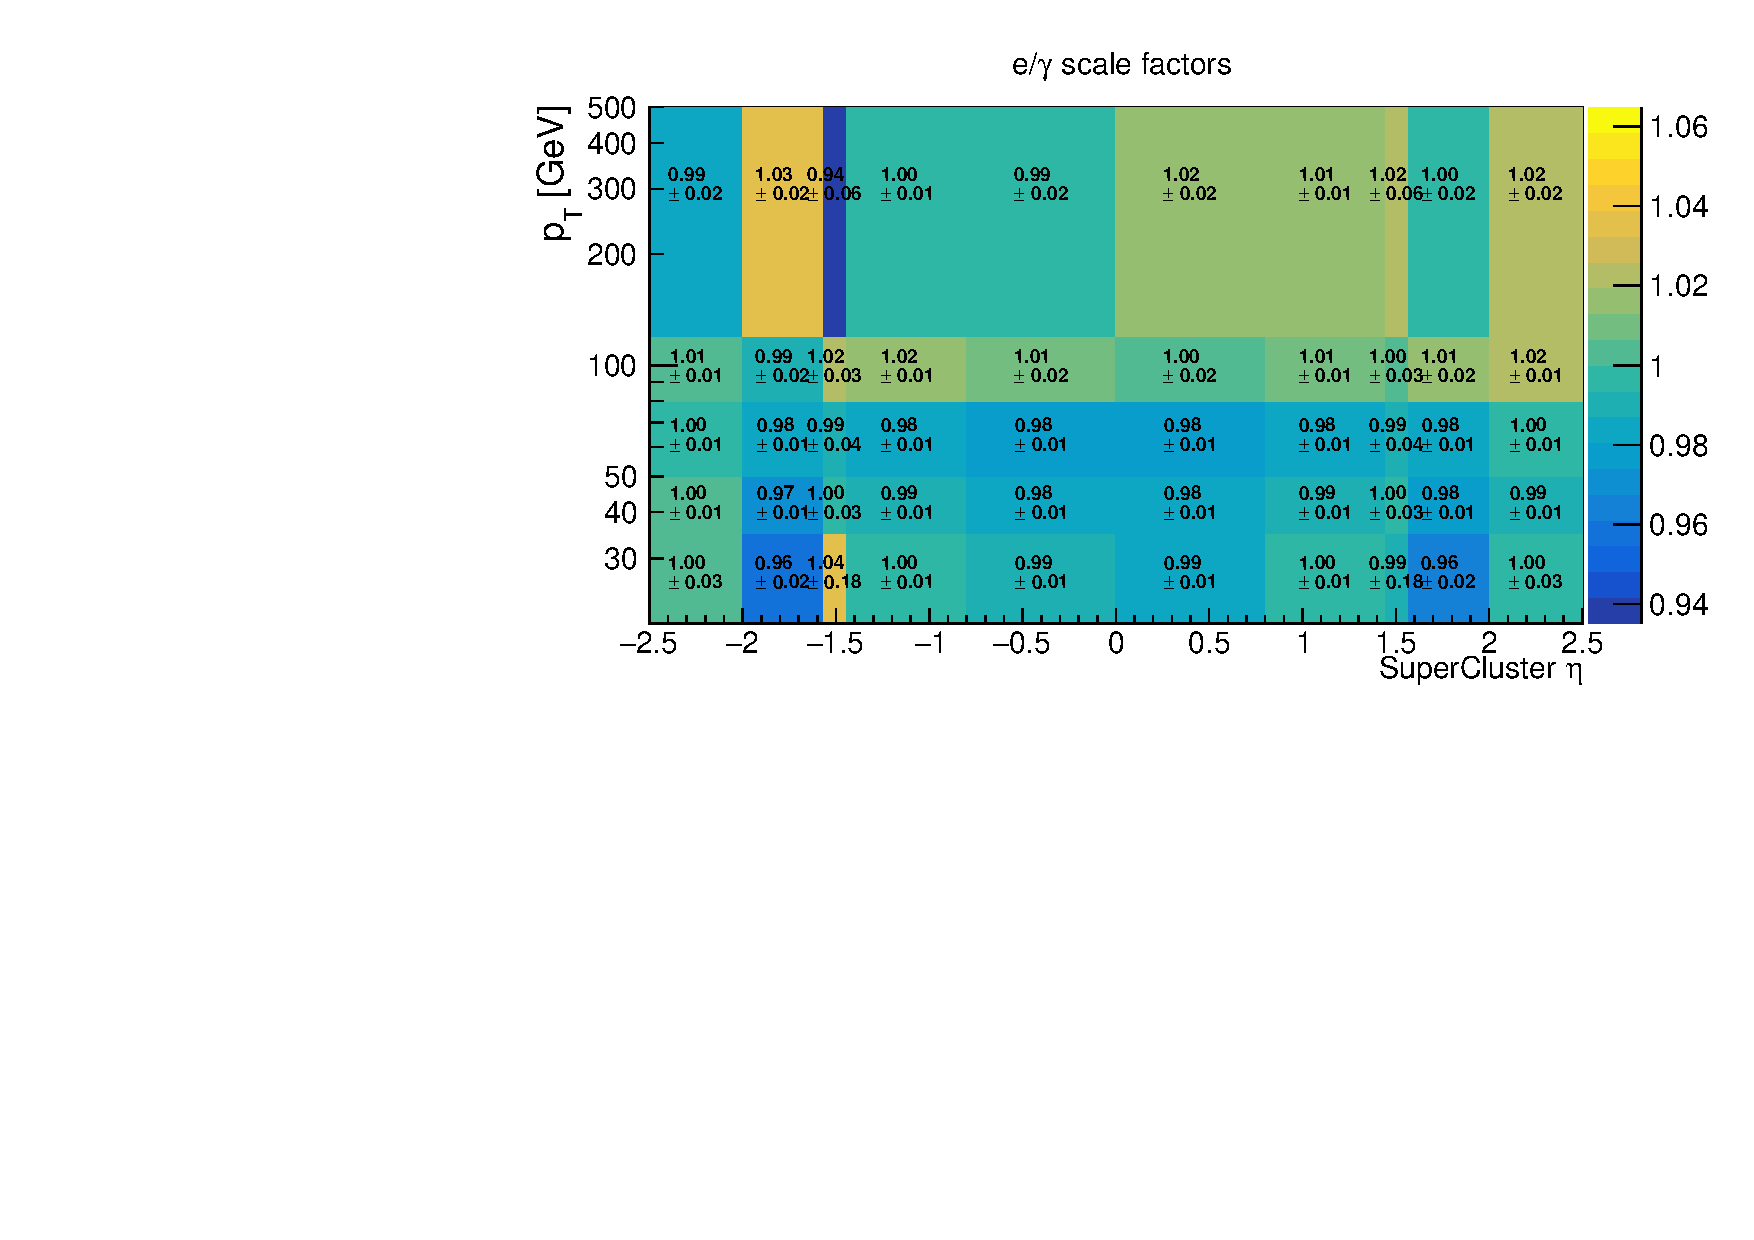
\includegraphics[width=.5\textwidth]{SF/phEffSF_2016preVFP.pdf} }}
  \subfigure [2016postVFP] {\resizebox{.5\textwidth}{!}{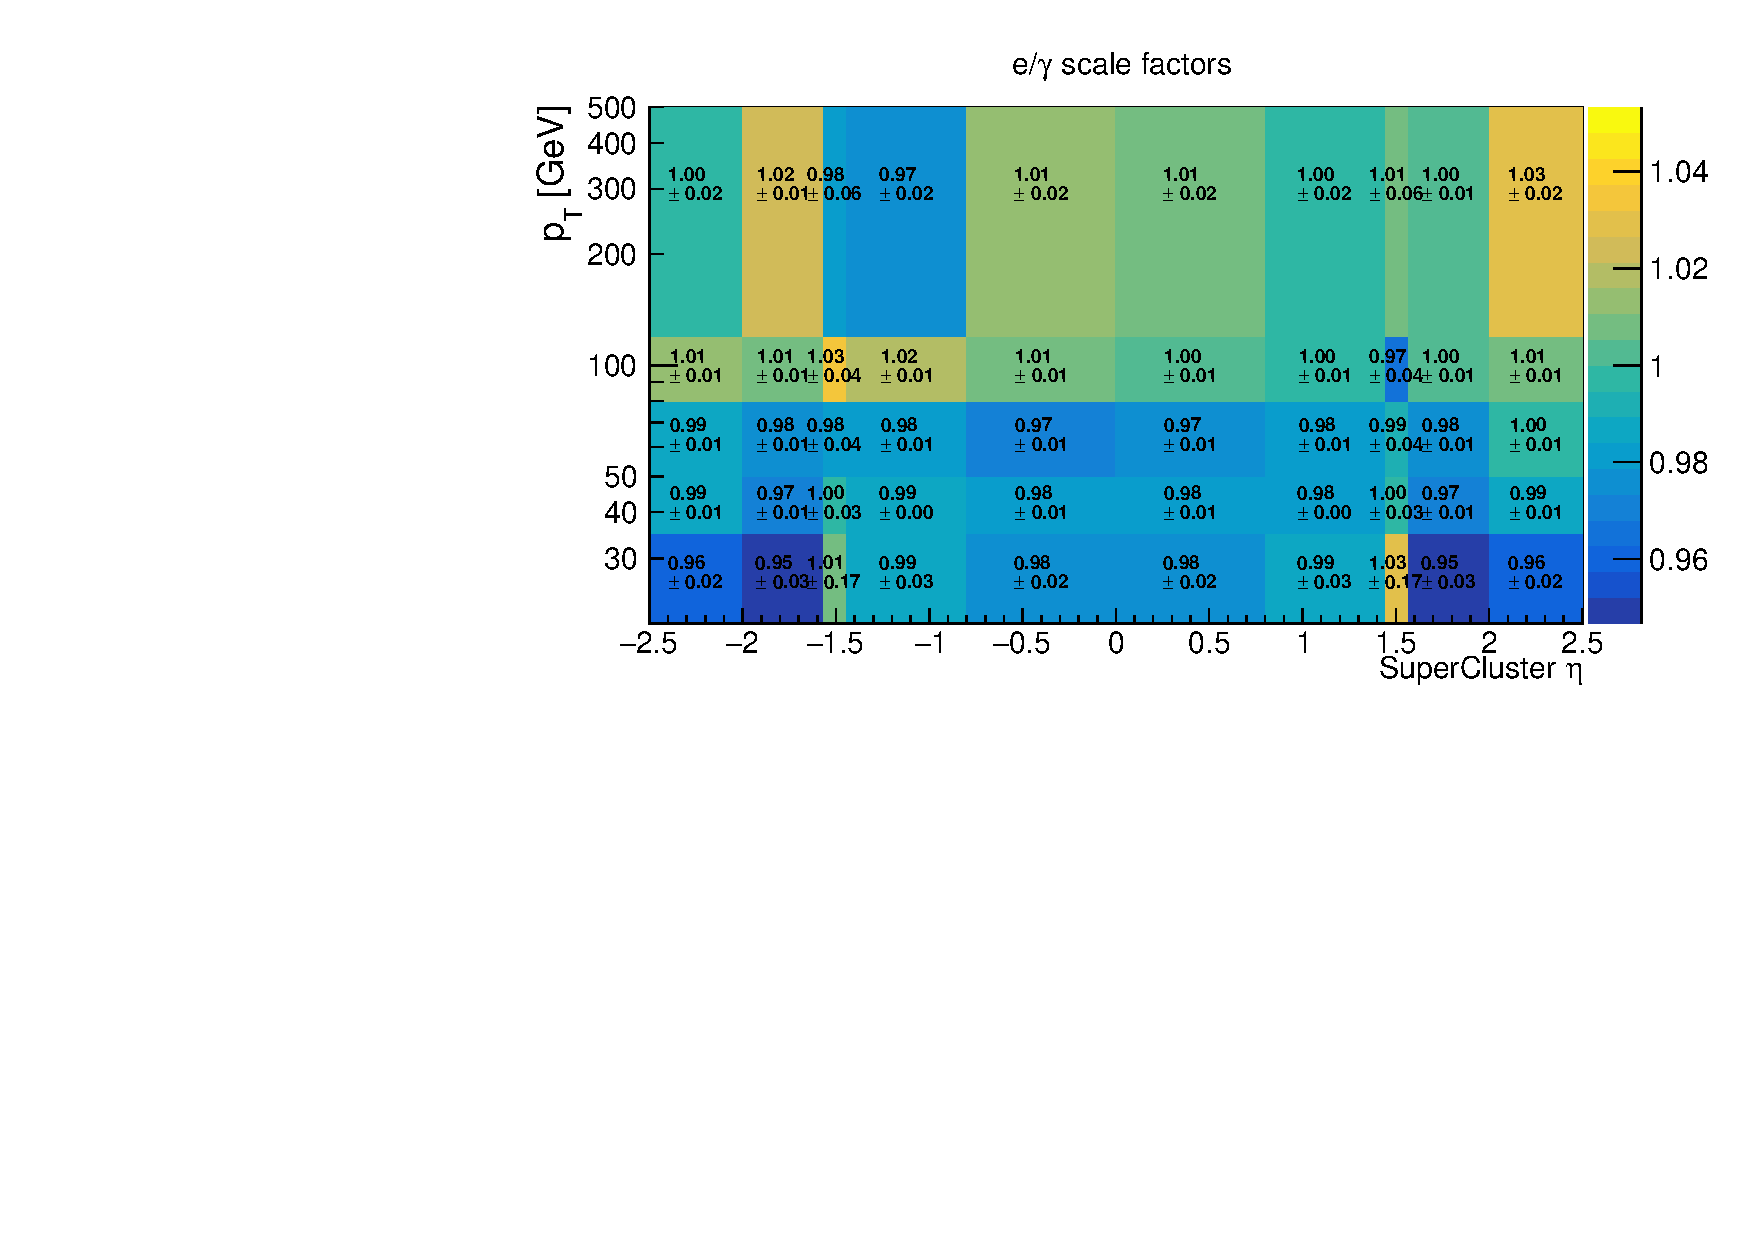
\includegraphics[width=.5\textwidth]{SF/phEffSF_2016postVFP.pdf}}}\\
  \subfigure [2017]        {\resizebox{.5\textwidth}{!}{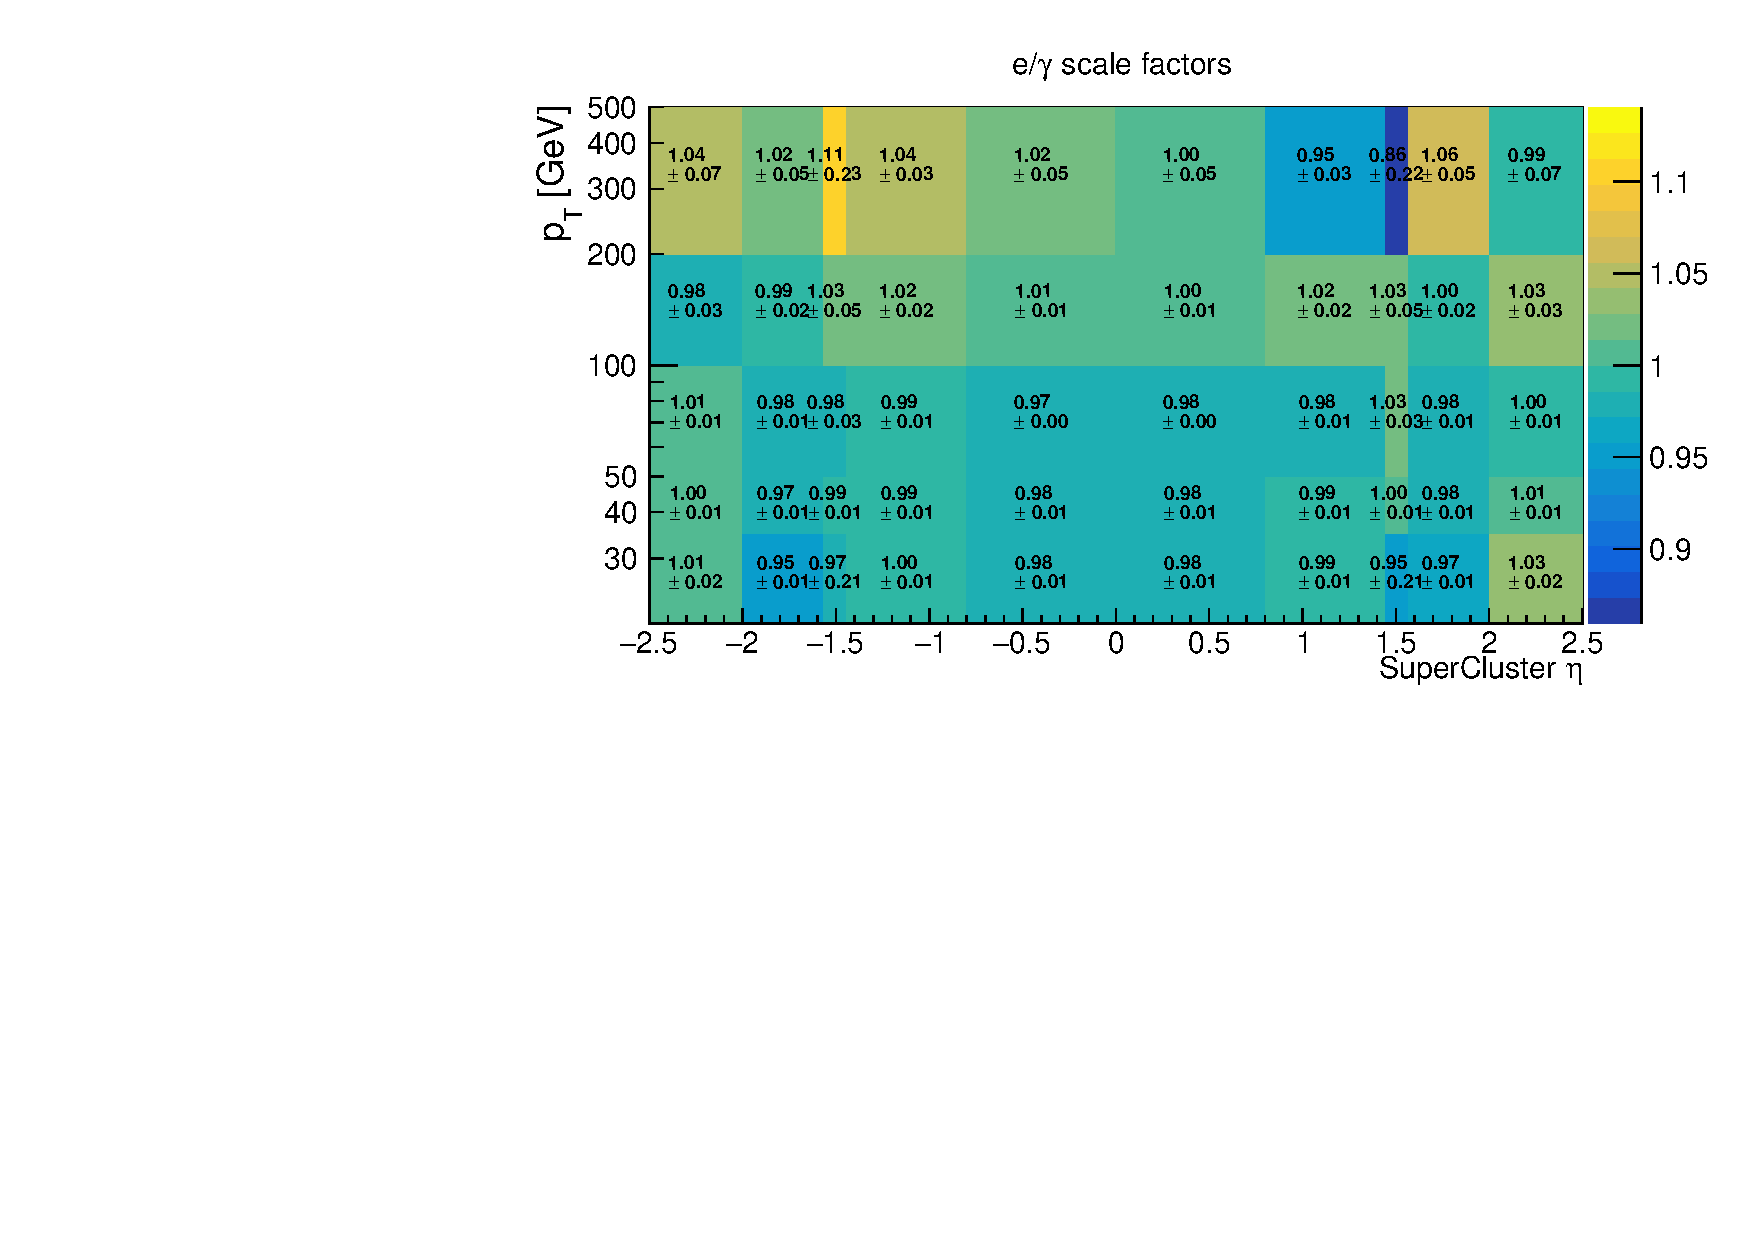
\includegraphics[width=.5\textwidth]{SF/phEffSF_2017.pdf}}}
  \subfigure [2018]        {\resizebox{.5\textwidth}{!}{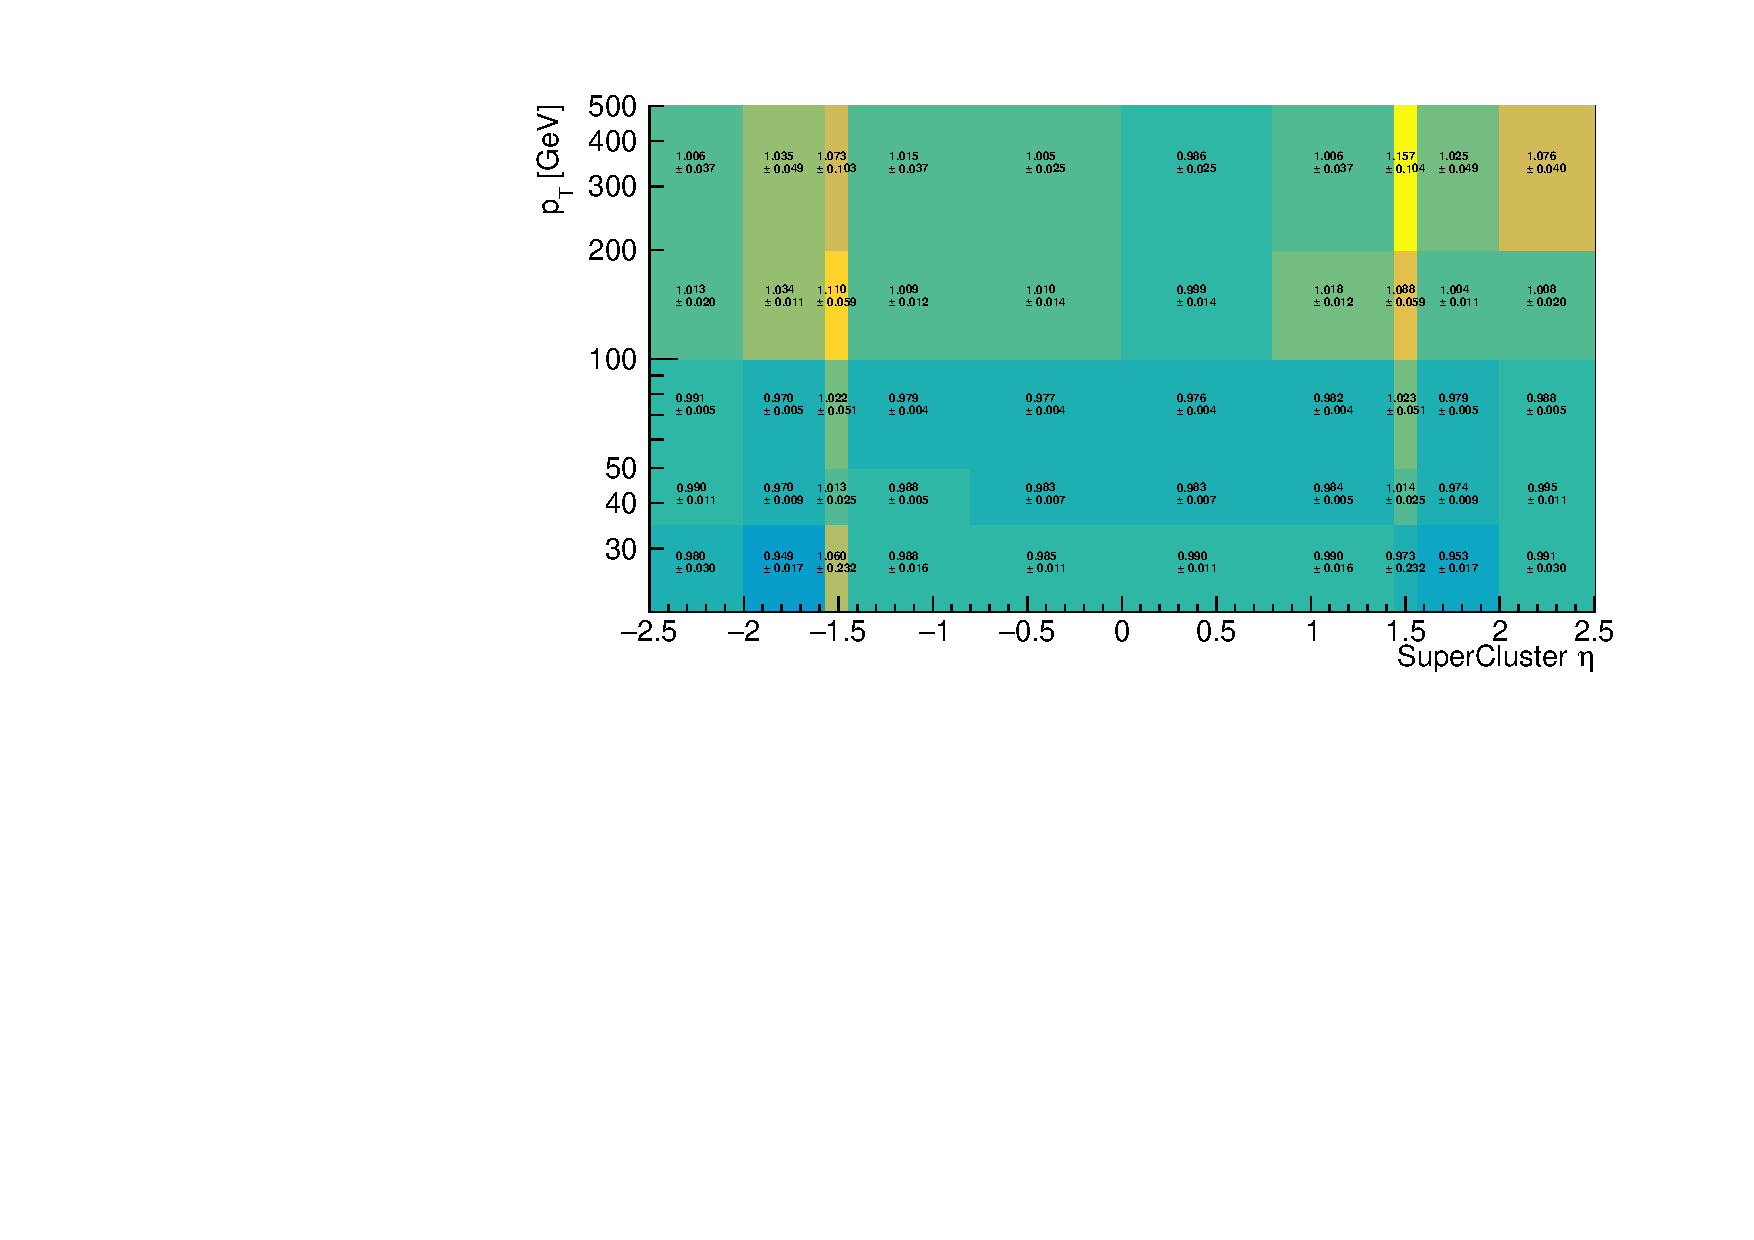
\includegraphics[width=.5\textwidth]{SF/phEffSF_2018.pdf}}}
  \caption{Photon efficiency scale factors for the cut-based Loose ID.}
  \label{fig:phEffSF}
\end{figure}

Besides the identification working points, an electron veto selection (CSEV veto) is also applied.
%% The scale factors are shown in ~\ref{tab:eleveto_SFs}.

%% \begin{table}[htbp]
%%  \centering
%%    \begin{tabular}{|c|c|l|l|}
%%    \hline
%%    Year & $p_T$& barrel & endcap\\ \hline
%%    2016 & inclusive &0.9938 $\pm$ 0.0119 & 0.9875 $\pm$ 0.0044\\\hline
%%    2017 & inclusive & 0.9862 $\pm$ 0.0030 & 0.9638 $\pm$ 0.0047\\\hline
%%    \multirow{3}{*}{2018} &10 GeV$<p_{T}^{\gamma}<30$ GeV &0.9869 $\pm$ 0.0043& 0.9535 $\pm$ 0.0054\\
%%    & 30 GeV$<p_{T}^{\gamma}<$60 GeV  &0.9908  $\pm$ 0.0111 & 0.9646 $\pm$ 0.0076\\
%%    & 60 GeV$<p_{T}^{\gamma}<$200 GeV &1.0084  $\pm$ 0.0856& 1.0218 $\pm$ 0.1178\\
%%    \hline
%%    \end{tabular}
%%    \caption{Electron veto scale factors for barrel and endcap corresponding to 2016 to 2018.}
%%    \label{tab:eleveto_SFs}
%%  \end{table}

%\begin{figure}[b]
%  \begin{center}
%    \includegraphics[width=0.8\textwidth]{figs/photon_SFs.pdf}
%    \caption{Photon ID scale factors for cut-based loose Photon selection}
%    \label{fig:PhotonEff}
%  \end{center}
%\end{figure}

\paragraph{Multivariate ID\\}
A more sophisticated photon identification strategy, is based on a multivariate technique, based on a Boosted Decision Tree (BDT) \cite{CMS:EGM-17-001}.
This multivariate (MVA) discriminant is built based on 14 input variables,
and provides excellent separation between signal (prompt photons) and background from misidentified jets.
The signal is defined as reconstructed photons from a \PGg + jets simulated sample that are matched at generator level with prompt photons within a cone of size $\DR = 0.1$,
whereas the background is defined by reconstructed photons in the same sample that do not match with a generated photon.
Photon candidates with $\ET > 15 \GeV$, $|\eta| < 2.5$, and satisfying very loose preselection requirements are used for the training of the BDT.
The variables used include the energy and shower shape of the supercluster, as well as various isolations.
Some of these variables are also employed by the cut-based ID, so the two discriminants are not independent.
%% The full list is shown in Table~\ref{tab:MVAvariables}.
%% The version used is \texttt{RunIIFall17v2}.

%% \begin{table}[ht]
%% \caption[.]{Variables used by the MVA-based ID, version \texttt{RunIIFall17v2}}
%% \label{tab:MVAvariables}
%% \centering
%% \begin{tabular}{l|l}
%% Name & variable\\
%% \hline
%% SCRawE             & superCluster.rawEnergy                                               \\
%% r9                 & r9                                                                   \\
%% sigmaIetaIeta      & full5x5\_showerShapeVariables.sigmaIetaIeta                          \\
%% etaWidth           & superCluster.etaWidth                                                \\
%% phiWidth           & superCluster.phiWidth                                                \\
%% covIEtaIPhi        & full5x5\_showerShapeVariables.sigmaIetaIphi                          \\
%% s4                 & full5x5\_showerShapeVariables.e2x2/full5x5\_showerShapeVariables.e5x5\\
%% scEta              & superCluster.eta                                                     \\
%% rho                & fixedGridRhoAll                                                      \\
%% esEffSigmaRR       & full5x5\_showerShapeVariables.effSigmaRR                             \\
%% esEnergyOverRawE   & superCluster.preshowerEnergy/superCluster.rawEnergy                  \\
%% phoIso03           & photonIso                                                            \\
%% chgIsoWrtChosenVtx & chargedHadronIso                                                     \\
%% chgIsoWrtWorstVtx  & chargedHadronWorstVtxIso                                             \\
%% \end{tabular}
%% \end{table}

Two working points are provided centrally by the the dedicated group within CMS:
\texttt{wp90} and \texttt{wp80}, corresponding to 90 \% and 80 \% prompt photon efficiency respectively.
The cuts on the MVA estimator value that define the two working points are detailed in Table~\ref{tab:MVAwpCuts}.

\begin{table}[ht]
\caption[.]{Working points of the photon MVA-based ID, version \texttt{RunIIFall17v2}}
\label{tab:MVAwpCuts}
\centering
\begin{tabular}{lrr}
\toprule
Name & Barrel & Endcap \\
\midrule
\texttt{wp80} & -0.02 & -0.26 \\
\texttt{wp90} &  0.42 &  0.14 \\
\bottomrule
\end{tabular}
\end{table}

As with any other ID, to account for difference in the modelling of its efficiency in simulations and the true efficiency in data,
Scale Factors are measured for each year in different bins of \pt and $\eta$ for \texttt{wp80} (Figure \ref{fig:phEffMVASF_wp80}) and \texttt{wp90} (Figure \ref{fig:phEffMVASF_wp90}).

\begin{figure}
\centering
\subfigure [2016preVFP ] {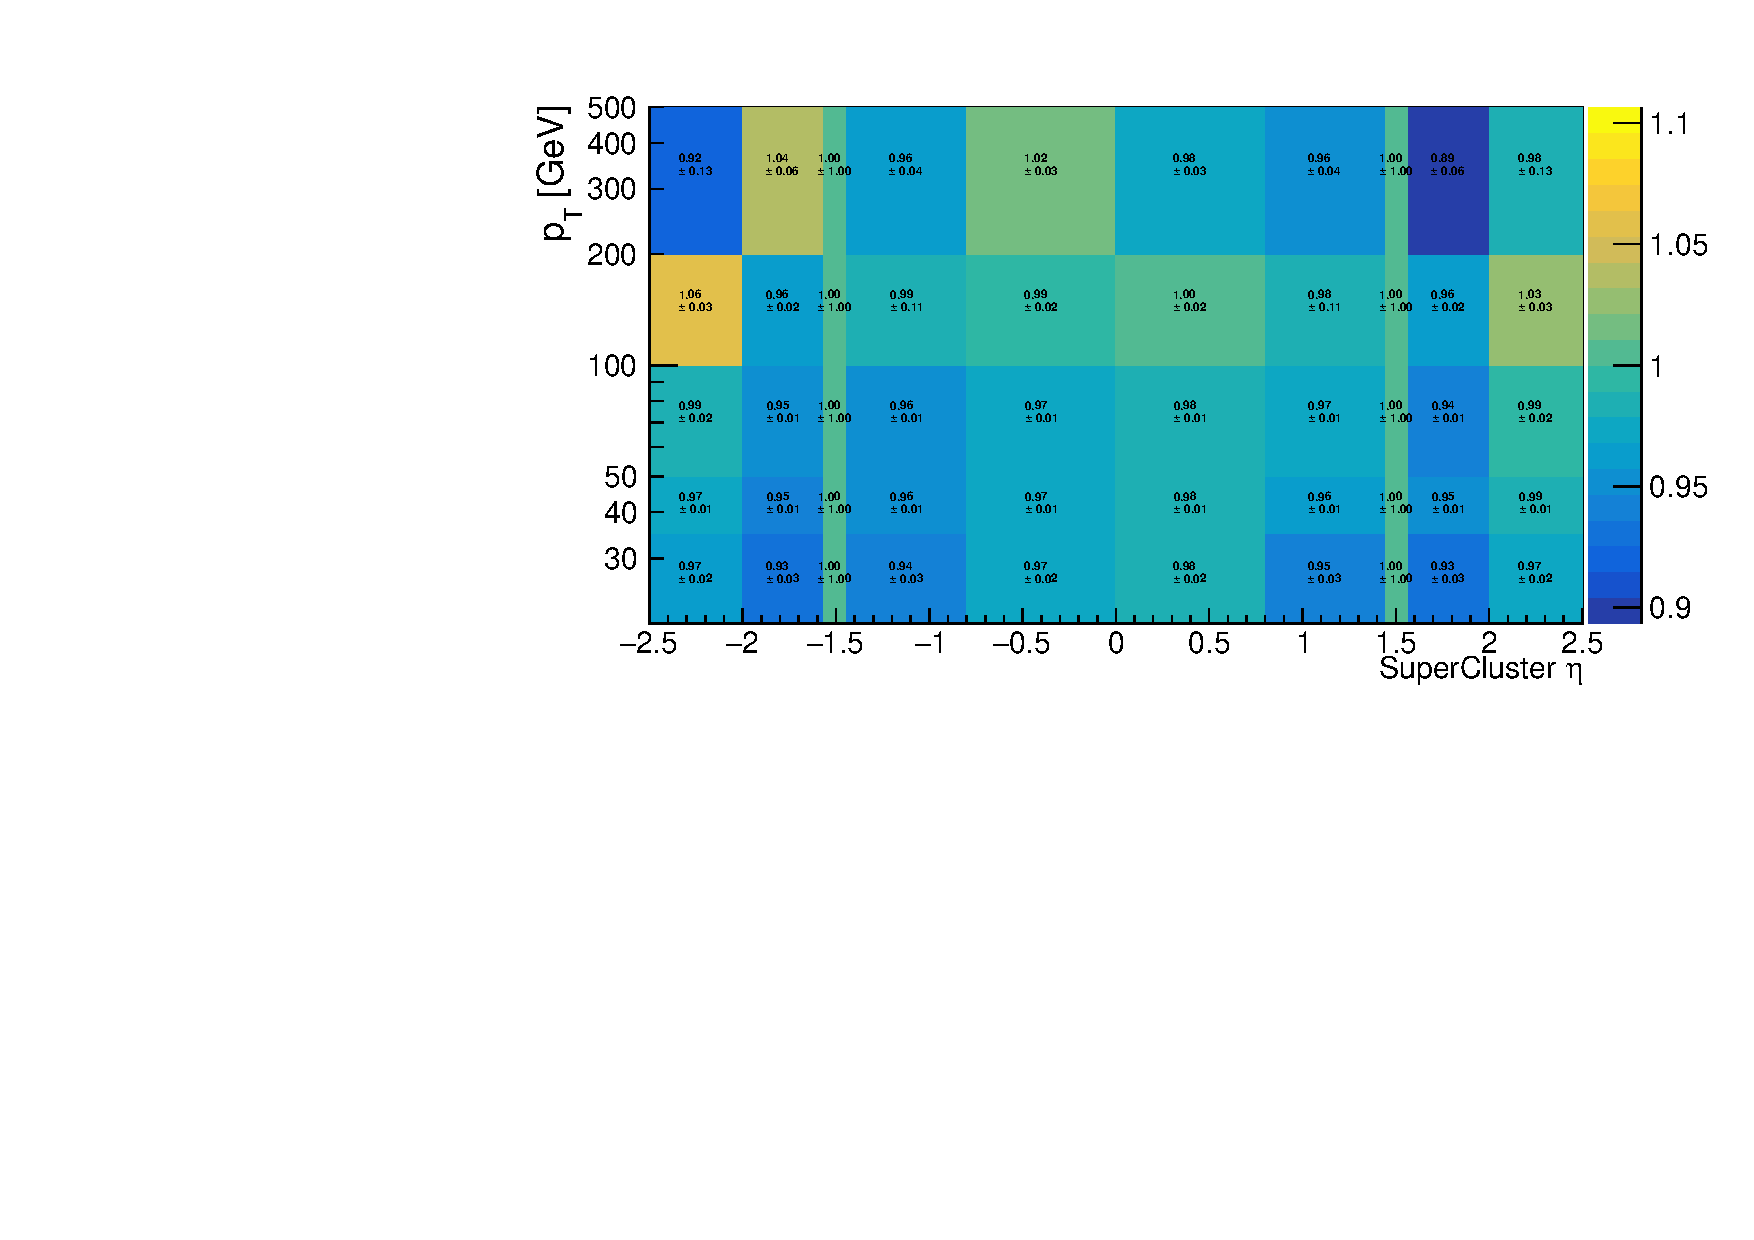
\includegraphics[width=.5\textwidth]{SF/2016_PhotonsMVAwp80_SF2D.pdf}}%
\subfigure [2017]        {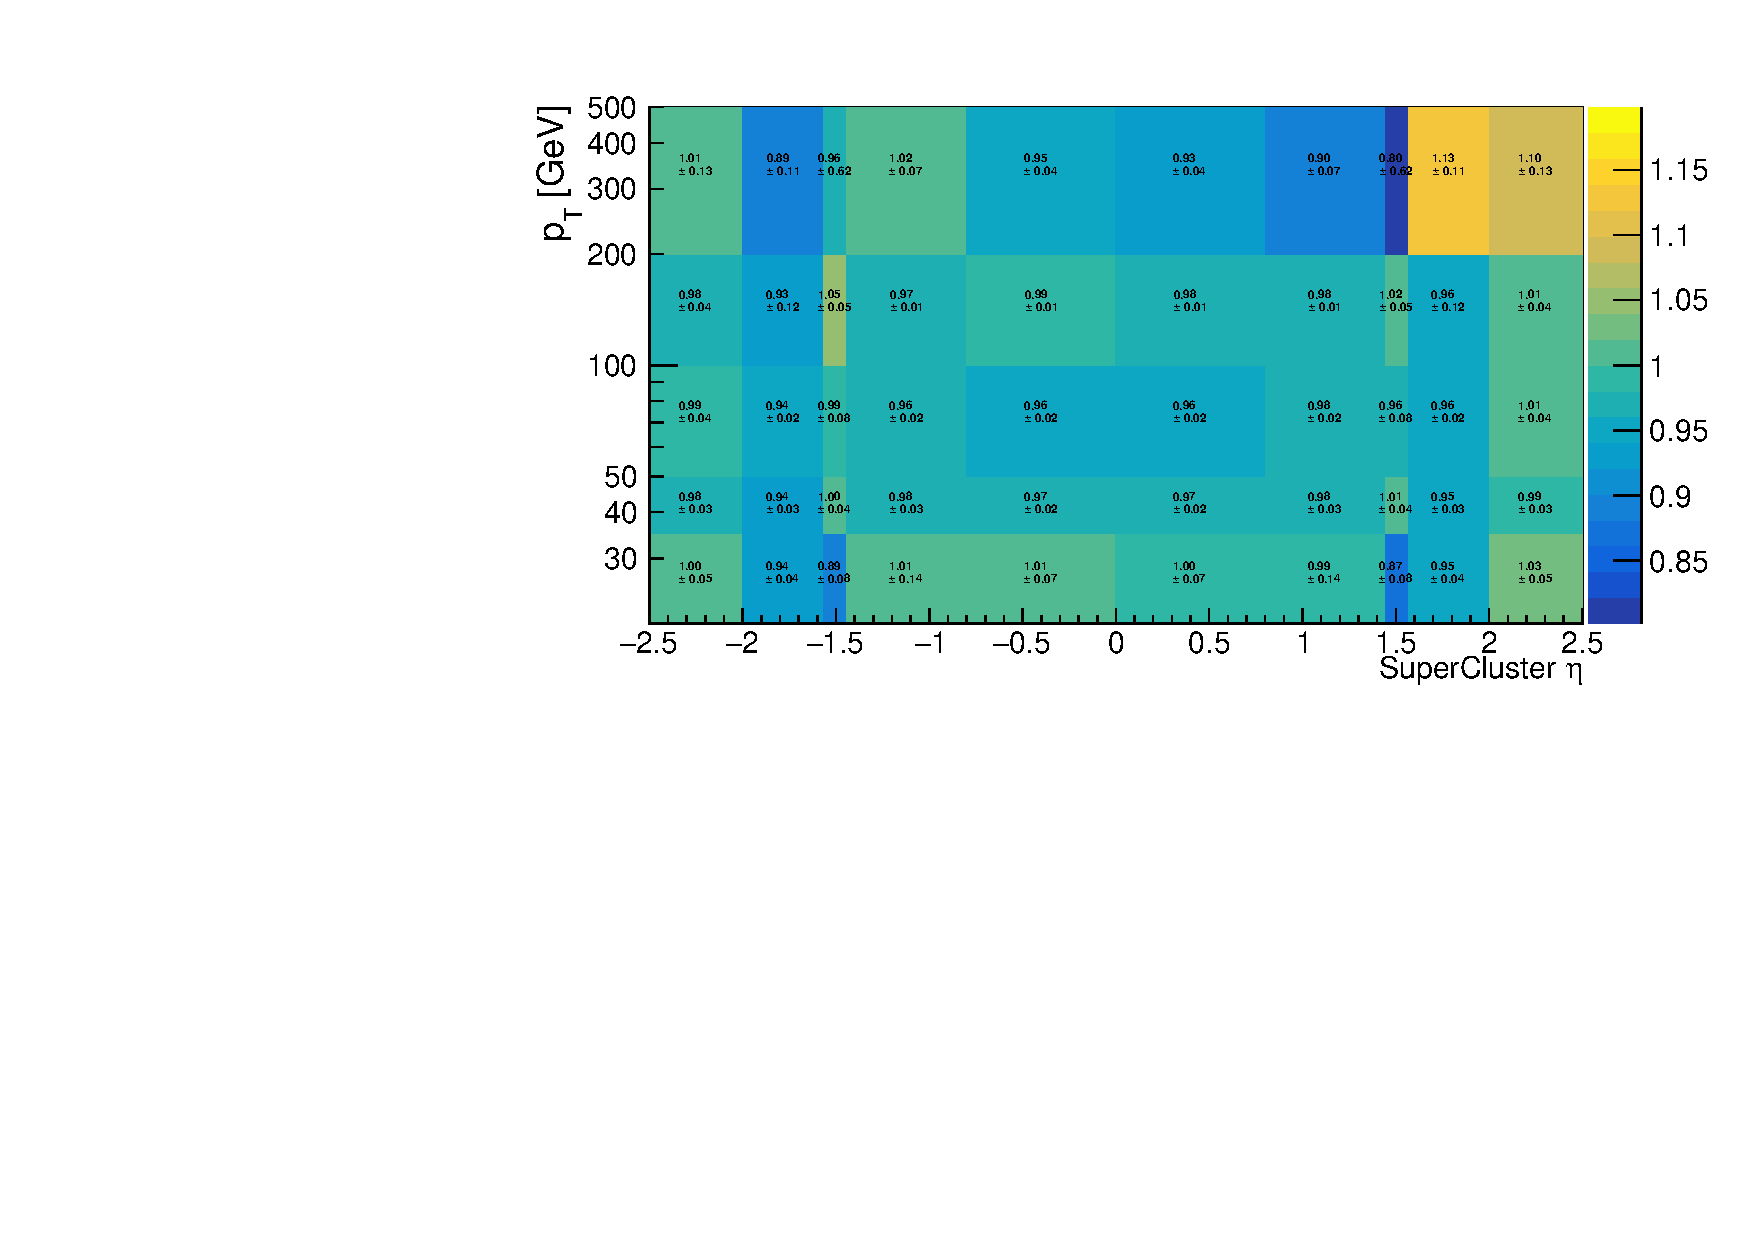
\includegraphics[width=.5\textwidth]{SF/2017_PhotonsMVAwp80_SF2D.pdf}}\\
\subfigure [2018]        {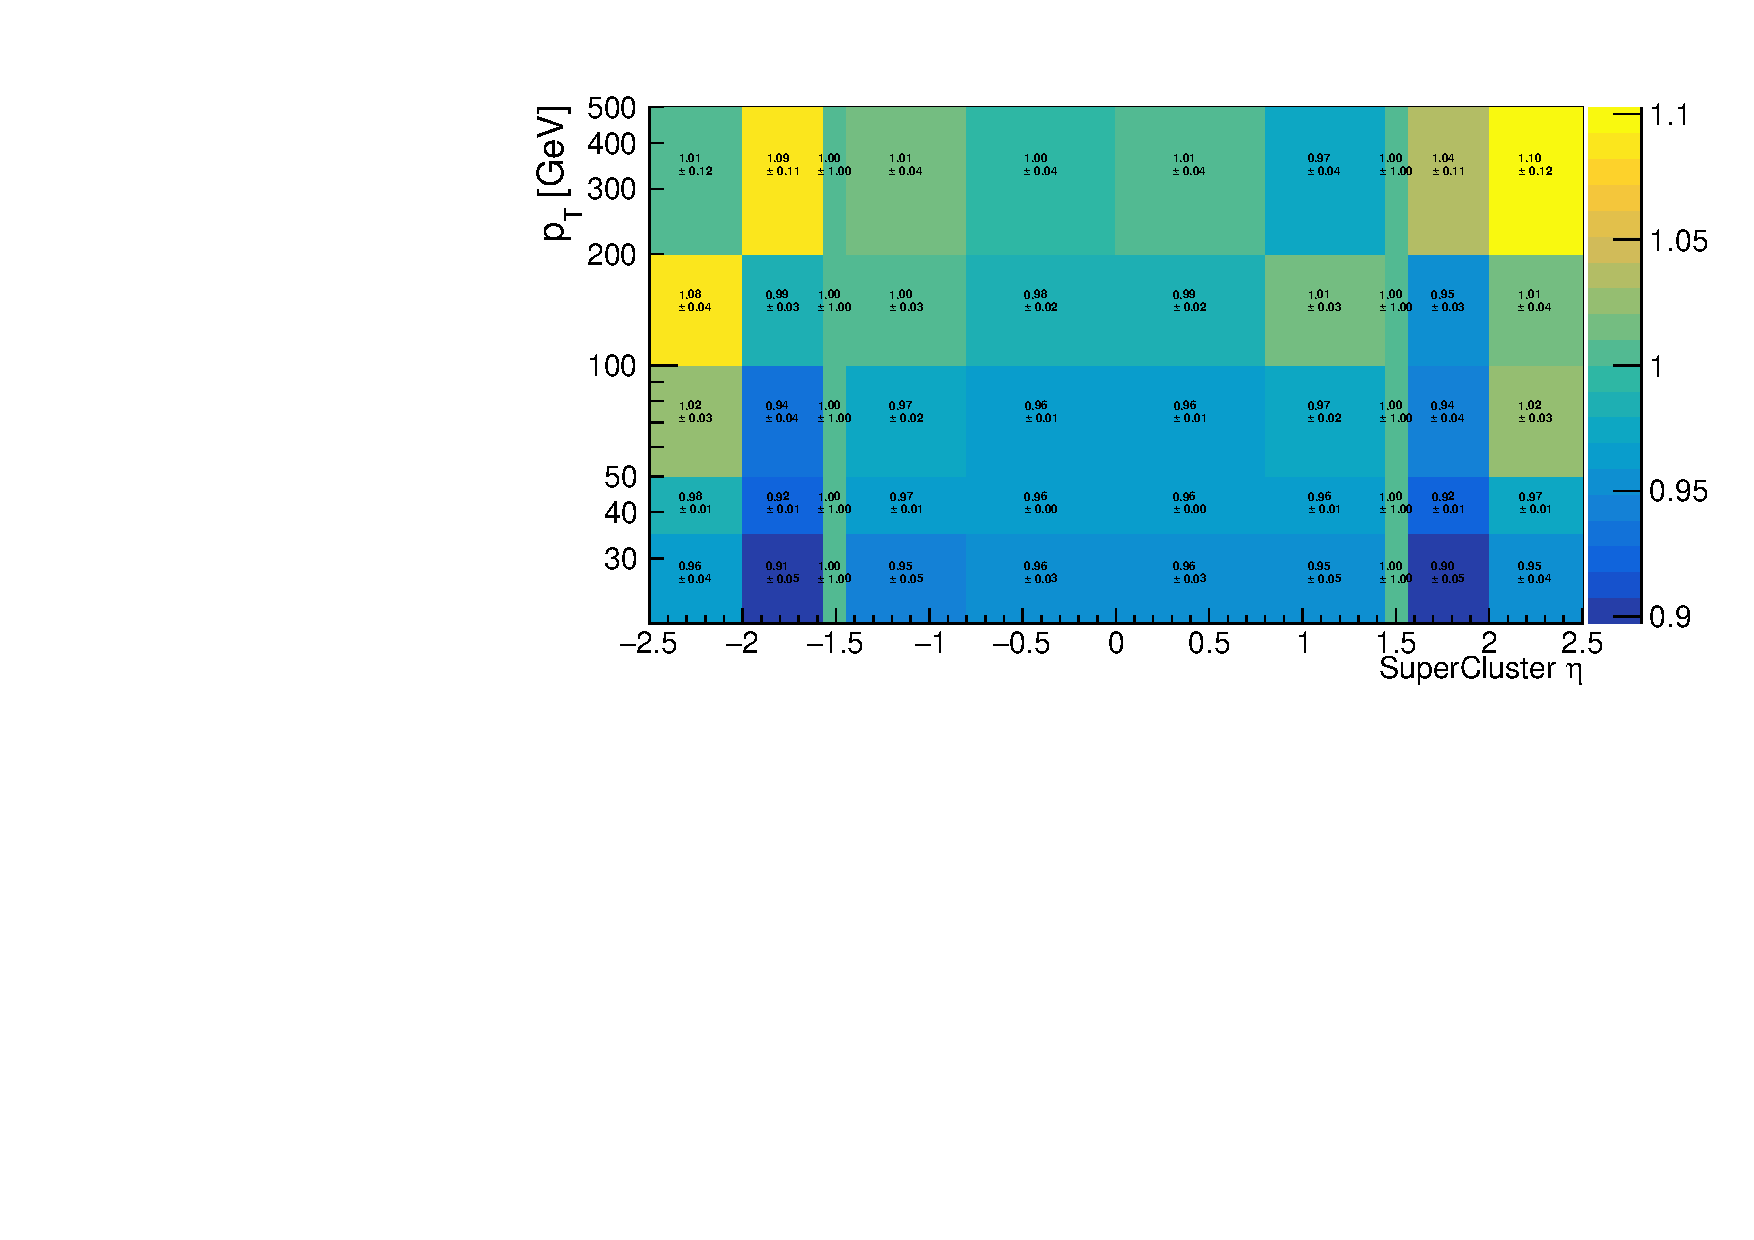
\includegraphics[width=.5\textwidth]{SF/2018_PhotonsMVAwp80_SF2D.pdf}}
\caption{Photon efficiency scale factors for the MVA-based ID with working point \texttt{wp80}.}
\label{fig:phEffMVASF_wp80}
%% }
\end{figure}

\begin{figure}
\centering
\subfigure [2016preVFP ] {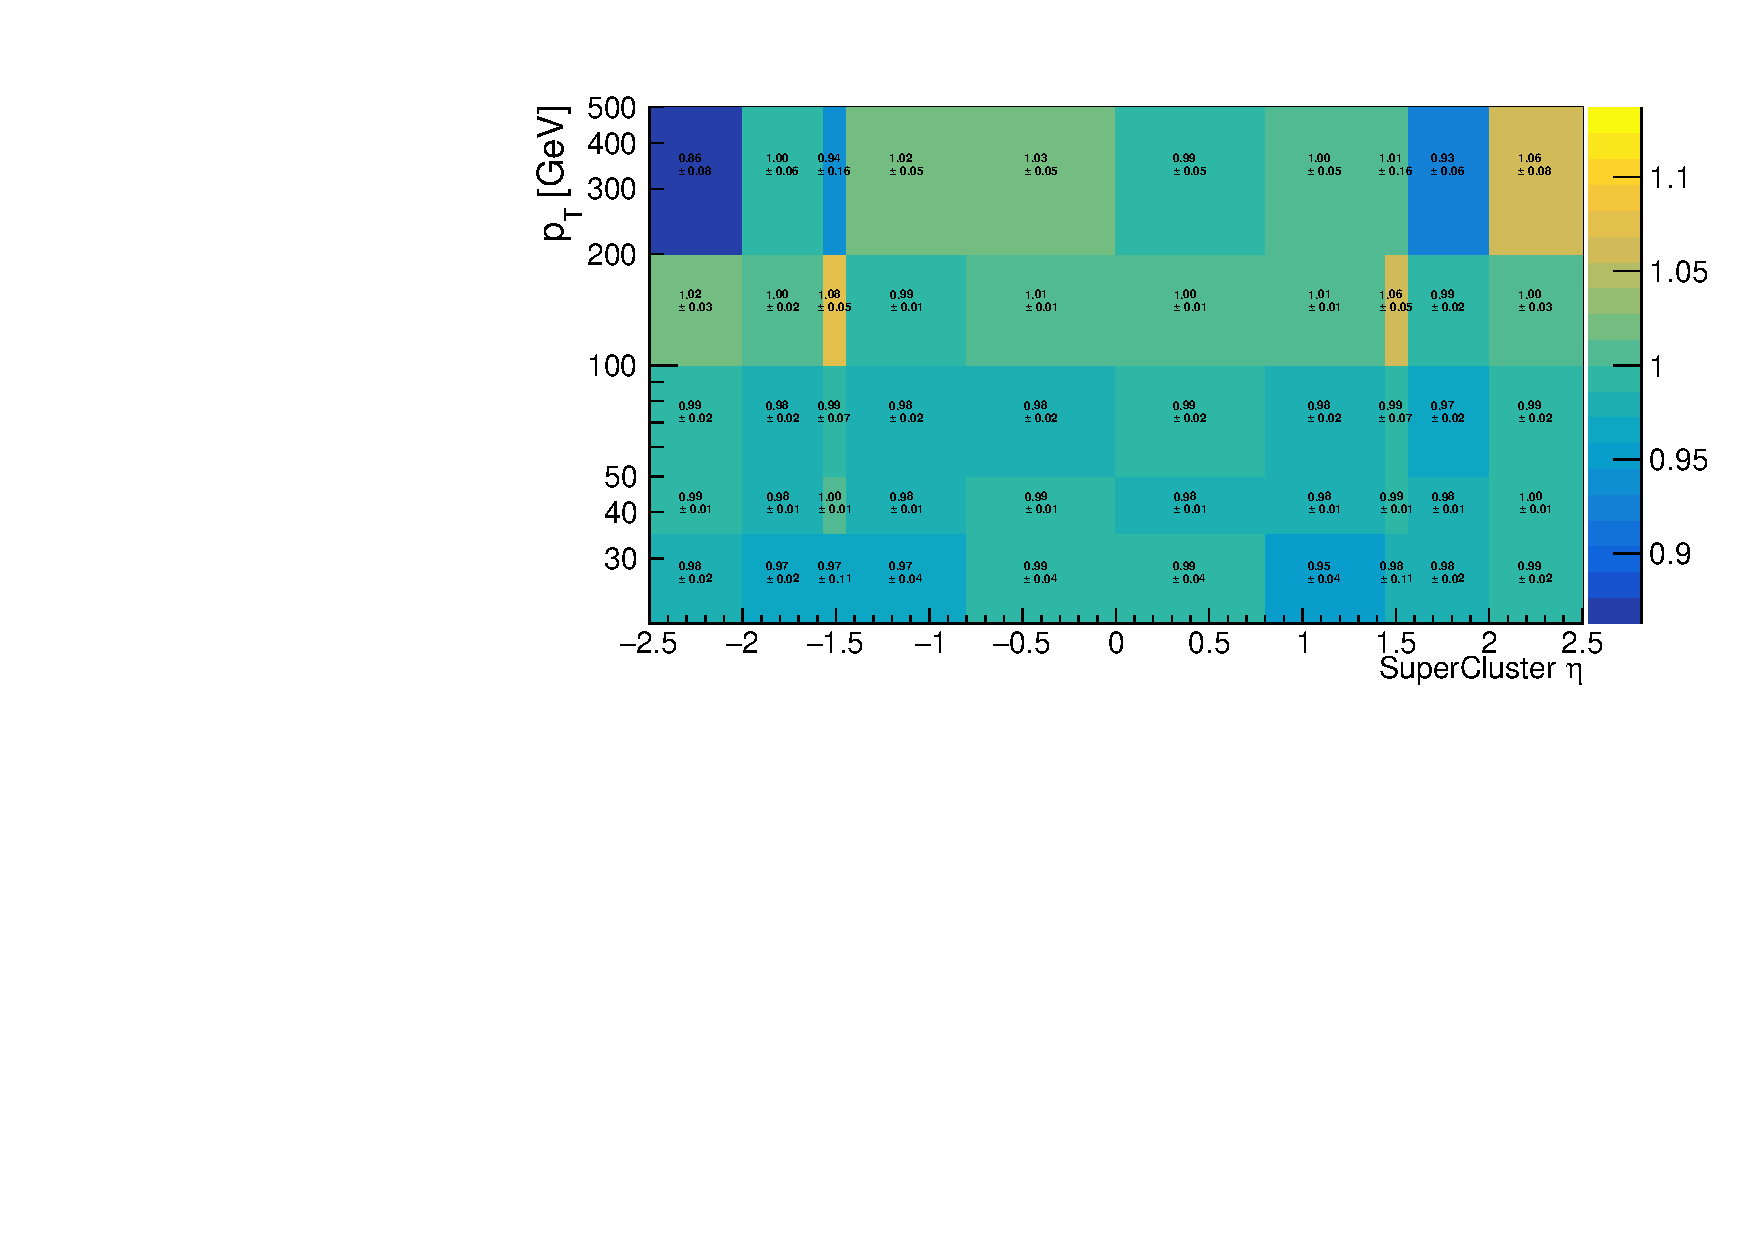
\includegraphics[width=.5\textwidth]{SF/2016_PhotonsMVAwp90_SF2D.pdf}}%
\subfigure [2017]        {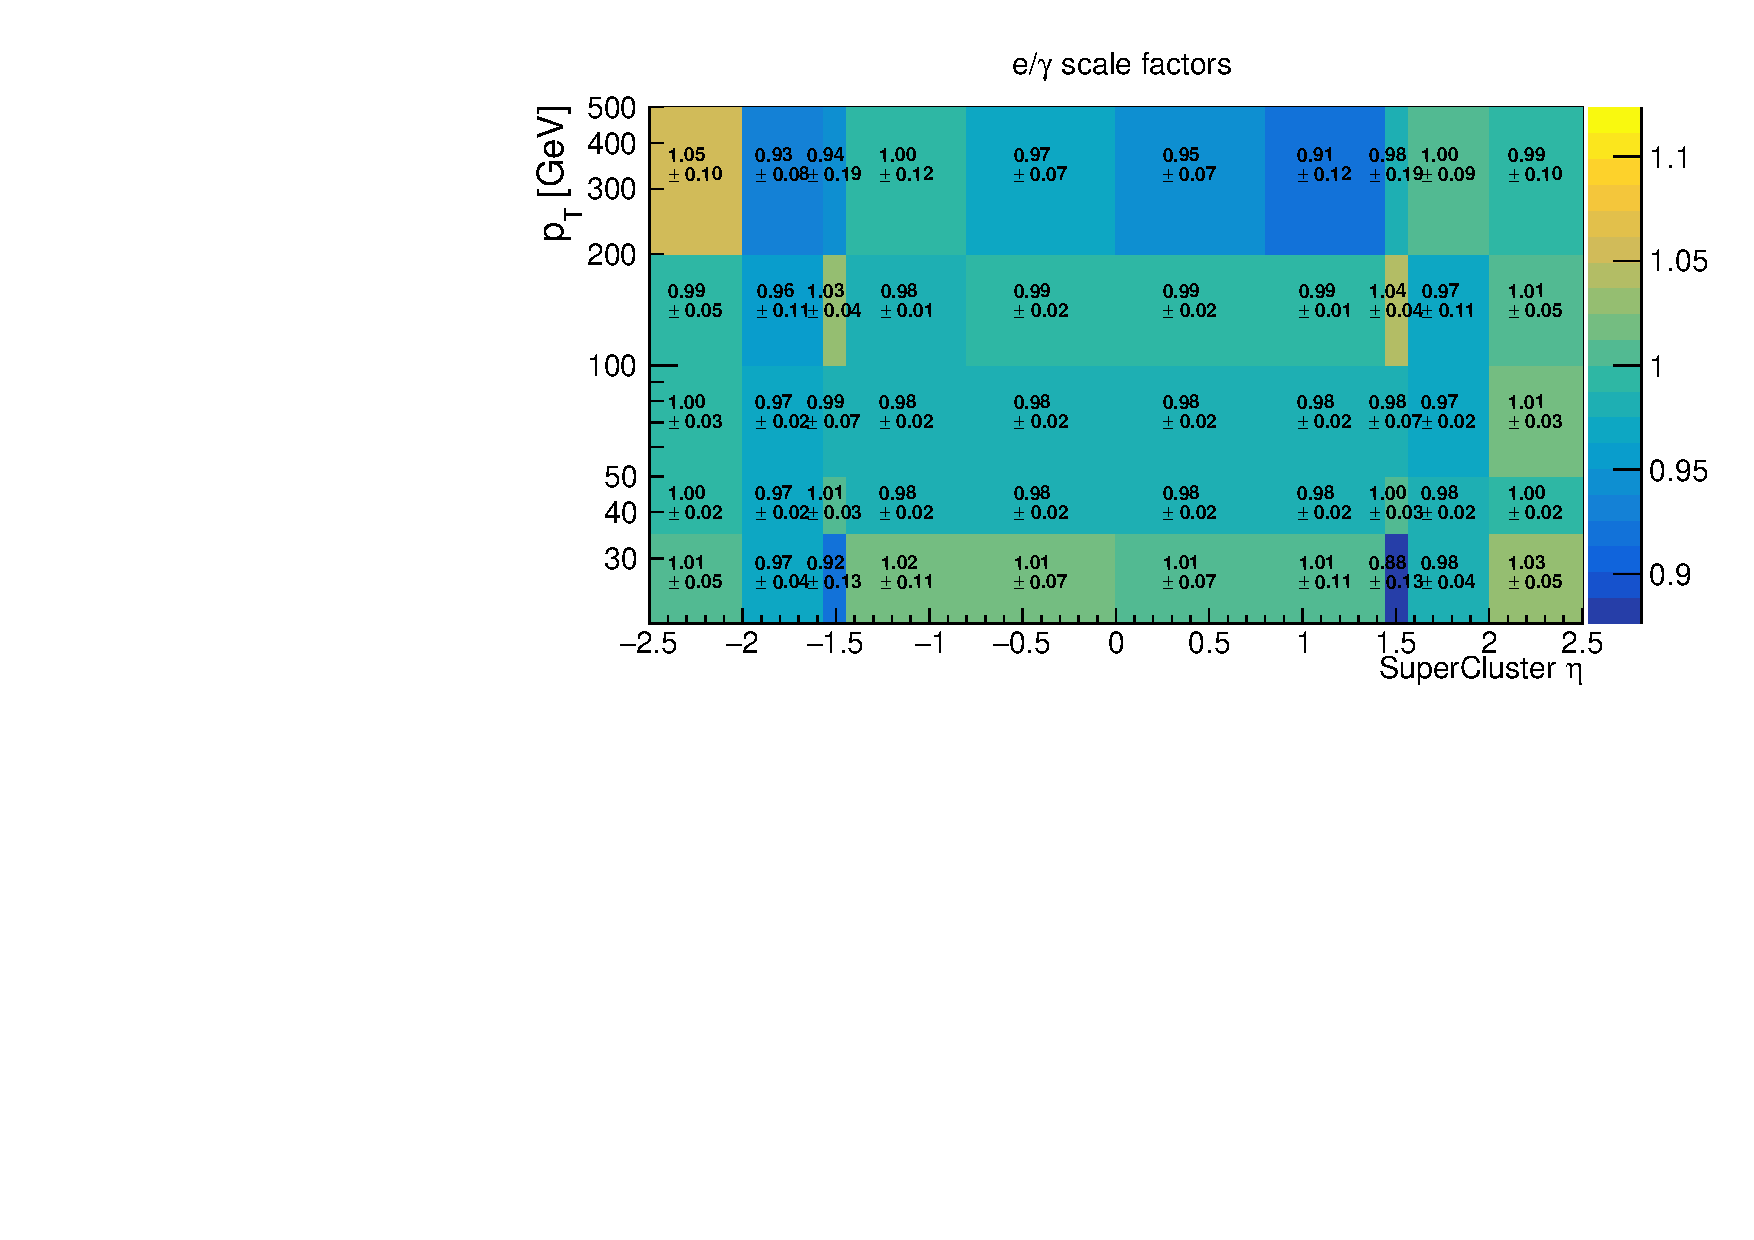
\includegraphics[width=.5\textwidth]{SF/2017_PhotonsMVAwp90_SF2D.pdf}}\\
\subfigure [2018]        {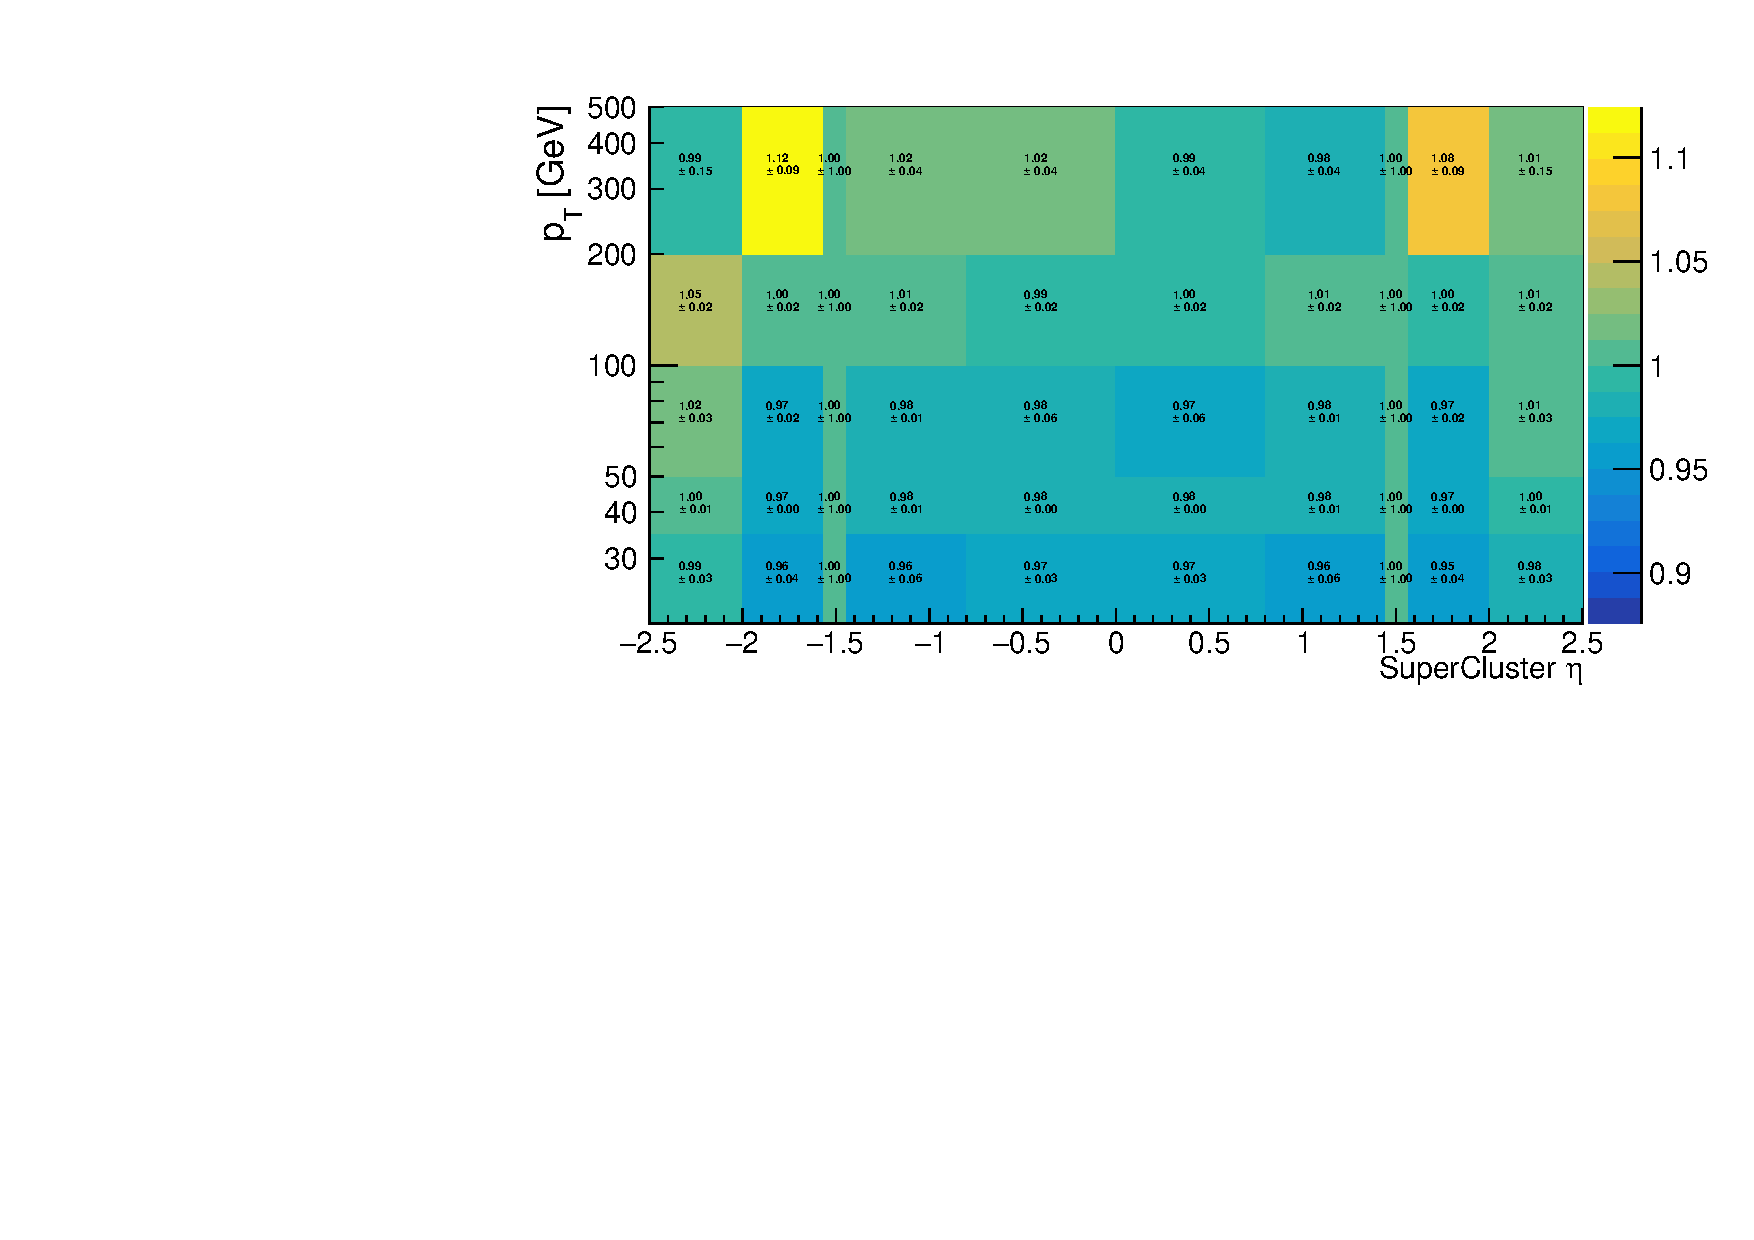
\includegraphics[width=.5\textwidth]{SF/2018_PhotonsMVAwp90_SF2D.pdf}}
\caption{Photon efficiency scale factors for the MVA-based ID with working point \texttt{wp90}.}
\label{fig:phEffMVASF_wp90}
\end{figure}

A comparison between the cut-based and the MVA-based IDs is shown in Figure~\ref{fig:PhotonIsoAUC}.
It represent the background rejection as a function of the signal efficiency for the raw MVA discriminant
and the three working points of the cut-based ID.

\begin{figure}
\centering
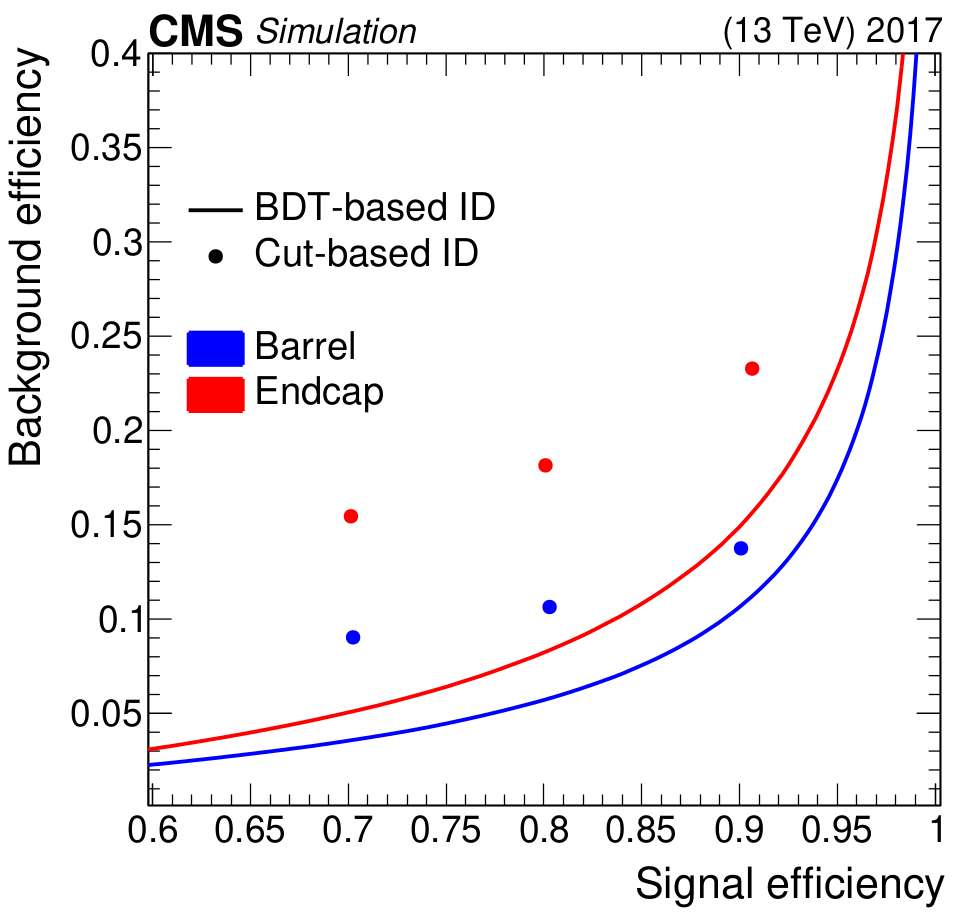
\includegraphics[width=.5\textwidth]{PhotonIsoAUC.png}
\caption{Performance of the photon BDT and cut-based identification algorithms in 2017.
Three different working points (loose, medium and tight) are shown for the cut-based ID. \cite{CMS:photon-performance-2015}}
\label{fig:PhotonIsoAUC}
\end{figure}

\paragraph{Selections used in the analysis\\}
\label{sec:photon_selection}

A common base selection is applied to all the photons, consisting of
\pt > 20 \GeV and
$|\eta| < 1.4442$ OR $1.566 < |\eta| < 2.4$.
Photons must also pass a conversion safe electron veto (CSEV) \cite{CMS:photon-performance-2015} which requires the absence of charged particle tracks,
with a hit in the innermost layer of the pixel detector not matched to a reconstructed conversion vertex, pointing to the photon cluster in the ECAL.
Photons are also rejected in the presence of a seed in the pixel tracker consisting of at least two hits,
which points to the ECAL within some window defined around the photon SC position.
Photons that pass these selections are called \textbf{kinematic photons}, which is the loosest selection used in this analysis.

Photons that also pass the cut thresholds of the Loose cut-based ID (see Table~\ref{tab:VPhotonID}) for H/E, the neutral ($I_n$) and photon ($I_\PGg$) isolations
are defined \textbf{very loose} photons.
They are used as the loose working point in a tight-to-loose method (Section \ref{sec:fake_photons_background}) to estimate the \nonprompt photon background.

The photons that also pass the \sieie and charged isolation ($I_{ch}$), and thus the Loose cut-based ID, are the \textbf{loose photons},
which is the tight selection for the \nonprompt photon background,
and the analysis selection for the results derived using the cut-based ID.

Additionally, kinematic photons that pass the MVA-based working points wp90 and wp80 are also considered,
given the improved performance of the MVA ID over the cut-based one.
The drawback of this ID is that it is not possible to do a data-driven estimation of the \nonprompt background,
due to the limited size of the application region defined by requiring a photon that passes the wp90 but fails the wp80,
as explained in Section~\ref{sec:fake_photons_background}.
